%Version 3.1 December 2024
% Site-Level Study on EU ETS Policy Effects on Satellite-Observed Air Quality
%%%%%%%%%%%%%%%%%%%%%%%%%%%%%%%%%%%%%%%%%%%%%%%%%%%%%%%%%%%%%%%%%%%%%%

\documentclass[pdflatex,sn-nature]{sn-jnl}% Math and Physical Sciences Numbered Reference Style

%%%% Standard Packages
\usepackage{graphicx}%
\usepackage{multirow}%
\usepackage{amsmath,amssymb,amsfonts}%
\usepackage{amsthm}%
\usepackage{mathrsfs}%
\usepackage[title]{appendix}%
\usepackage{xcolor}%
\usepackage{textcomp}%
\usepackage{manyfoot}%
\usepackage{booktabs}%
\usepackage{algorithm}%
\usepackage{algorithmicx}%
\usepackage{algpseudocode}%
\usepackage{listings}%
\usepackage{tikz}%
\usetikzlibrary{positioning,arrows.meta,shapes.geometric,fit,backgrounds}%

%% Theorem styles
\theoremstyle{thmstyleone}%
\newtheorem{theorem}{Theorem}%
\newtheorem{proposition}[theorem]{Proposition}%

\theoremstyle{thmstyletwo}%
\newtheorem{example}{Example}%
\newtheorem{remark}{Remark}%

\theoremstyle{thmstylethree}%
\newtheorem{definition}{Definition}%

\raggedbottom

\begin{document}

\title[EU ETS Effects on Emissions and Air Quality]{Quantifying the Effects of Climate Policy Stringency on Verified Emissions and Satellite-Derived NOx}
\subtitle{Master's Thesis}

\author*{\fnm{Arnav} \sur{Agrawal}}

\affil{\orgdiv{MA in Quantitative Methods in the Social Sciences}, \orgname{Columbia University}}

\abstract{I investigate how European Union Emissions Trading System (EU ETS) policy stringency affects verified CO$_2$ emissions, reported NOx emissions, and satellite-derived NOx proxies at 521 large combustion plants across Europe (2018--2023). Using two-way fixed effects with facility and region-by-year fixed effects, I find that a 10\% allocation shortfall is associated with 1.9\% lower verified CO$_2$ emissions ($\beta = -0.186$, $p < 0.001$) and 0.7\% lower reported NOx ($\beta = -0.066$, $p = 0.023$). Crucially, continuous interaction models reveal that treatment effects are \textit{fuel-dependent}: coal-dominant facilities show the strongest response ($\beta_{\text{coal}} = -0.62$ for CO$_2$, $-0.88$ for NOx), followed by oil and gas, while biomass facilities show no significant response. This pattern---where policy effectiveness depends on combustion technology rather than facility size or location---suggests carbon pricing operates primarily through fuel-specific abatement incentives. Satellite-derived NOx from TROPOMI, constructed via Beirle-style flux-divergence with a modified 5~km integration radius, shows null main effects at the permissive 0.01~kg/s detection limit due to measurement noise, but provides corroborative evidence through similar fuel-dependent heterogeneity patterns. The framework makes three methodological contributions: (i) geospatial foundation model embeddings (Google AlphaEarth) as high-dimensional controls for satellite retrieval confounders; (ii) NUTS2 regional clustering for inference with PyPSA-Eur power system clusters for electricity-sector heterogeneity; and (iii) a simplified Beirle-style NOx quantification method adapted for panel econometrics. The triple-outcome approach enables cross-validation: directional agreement between administrative CO$_2$ and reported NOx, with consistent heterogeneity patterns across all three outcomes, strengthens confidence in the fuel-dependent policy mechanism.}

\keywords{Climate Policy, Climate Monitoring, EU ETS, Verified Emissions, Satellite Remote Sensing, TROPOMI, NOx Emissions, Flux Divergence, Difference-in-Differences, Causal Inference, Large Combustion Plants}

\maketitle

%% ========================================================================
%% INTRODUCTION
%% ========================================================================
\section{Introduction}\label{sec:intro}

Evaluating climate policy requires measuring actual emission outcomes. The European Union Emissions Trading System (EU ETS) generates rich administrative data on verified CO$_2$ emissions at the installation level, providing the gold standard for measuring greenhouse gas output from regulated facilities. However, relying solely on self-reported emissions raises questions about verification and leaves unmeasured the local air quality co-benefits that accompany carbon reductions. Satellite remote sensing offers an independent, physically-grounded approach to quantifying emissions from space, potentially revealing both verification opportunities and co-pollutant dynamics that administrative data cannot capture.

This study adopts a triple-outcome approach that exploits the complementary strengths of administrative and satellite data. The three outcomes are: (i) verified EU ETS CO$_2$ emissions---high-quality, installation-level measures from the EU ETS registry that provide accurate compliance trajectories and absolute emission levels; (ii) reported NOx emissions from the Large Combustion Plant (LCP) Directive---administrative ground-truth for NOx that captures pollution co-benefits; and (iii) a satellite-derived NOx emission proxy---a physically grounded indicator constructed from TROPOMI NO$_2$ tropospheric columns and ERA5 winds, following the flux-divergence approach of Beirle et al. \cite{beirle2019,beirle2021,beirle2023}.

Why use three outcomes? CO$_2$ is a well-mixed greenhouse gas with global climate impacts; nitrogen
oxides (NO$_x$), by contrast, are criteria pollutants whose health effects---respiratory illness,
cardiovascular disease, premature mortality---fall disproportionately on populations living near
emission sources. Air quality co-benefits are particularly policy-relevant because they are local
and immediate, whereas averted climate damages are global and long-term. The triple-outcome design
provides: (i) verified CO$_2$ emissions for accurate carbon policy effect estimation, (ii) reported
NOx for ground-truth measurement of air quality co-benefits, (iii) satellite-derived NOx for
independent validation that is robust to reporting compliance issues and captures local air quality
effects beyond stack emissions, and (iv) cross-validation opportunities where all three outcomes
should respond to common policy shocks.

This study develops a novel framework for evaluating climate policy impacts using both administrative emissions data and satellite remote sensing. I focus on the European Union Emissions Trading System (EU ETS), the world's largest carbon market, which creates economic incentives for industrial facilities to reduce CO$_2$ emissions through a cap-and-trade mechanism. The framework addresses two fundamental methodological challenges: (i) constructing a satellite-derived NOx emission proxy that is physically interpretable and appropriate for panel econometric analysis, and (ii) controlling for high-dimensional confounders that affect both policy exposure and emission outcomes.

The study makes three methodological contributions. The first two follow a recent trend in causal inference toward incorporating machine learning-derived features to address high-dimensional confounding \cite{chernozhukov2018,veitch2019,zimmert2018}; the third adapts an atmospheric physics method for panel econometrics.

\textbf{First}, I demonstrate the use of geospatial foundation model embeddings as high-dimensional controls in panel-based climate monitoring studies. Specifically, I incorporate Google AlphaEarth embeddings \cite{alphaearth2025}---64-dimensional representations learned from multi-source satellite imagery, climate reanalysis, and geotagged text---as control variables in the econometric specifications. These embeddings capture between-unit heterogeneity arising from local geographic, infrastructural, and climate context in a data-efficient manner, providing a scalable approach to controlling for high-dimensional spatial confounders that would be impractical to specify manually. This application extends prior work on learned representations for causal inference---originally developed for text embeddings \cite{veitch2019}---to the domain of geospatial environmental monitoring. The approach is particularly suited to difference-in-differences settings where high-dimensional confounders may violate the parallel trends assumption if left uncontrolled \cite{zimmert2018}.

\textbf{Second}, I use Eurostat NUTS2 regions for spatial clustering in both fixed effects structure and inference. Standard errors are clustered by NUTS2 region, which groups facilities that share common regional economic conditions, labor markets, and policy enforcement mechanisms. The same regions define Region$\times$Year fixed effects, absorbing time-varying regional confounders that correlate with both policy exposure and air quality outcomes. Unlike sector-specific clustering (e.g., power system network clusters), NUTS2 regions apply uniformly to all industrial facility types and correspond to administrative units where EU and national environmental policies are implemented. For electricity sector heterogeneity analysis, I additionally implement PyPSA-Eur power system clusters \cite{horsch2018}---k-means clusters computed on transmission network topology---which group facilities facing correlated wholesale prices and dispatch patterns.

\textbf{Third}, for the satellite outcome, I implement a simplified Beirle-style flux-divergence method that provides physically grounded NOx emission estimates at the facility level. The approach computes the advection---the scalar product of wind velocity and the spatial gradient of NO$_2$ column density---which under the continuity equation is proportional to local emissions minus chemical loss. For each facility, I integrate advection over a 5 km disc (reduced from Beirle's standard 15 km based on validation against reported NOx emissions), apply a lifetime correction following \cite{beirle2023}, and convert to NOx emission rates. This methodology follows the Beirle et al. (2019, 2021, 2023) family of methods \cite{beirle2019,beirle2021,beirle2023}, which are physically transparent, computationally tractable for known point sources, and specifically designed for power-plant-scale NOx plumes.

The analysis links three data sources on large combustion plants (LCPs) in the EU: (i) the European Environment Agency's LCP registry providing plant characteristics and coordinates, (ii) EU ETS compliance data providing installation-level verified emissions and free allocations, and (iii) TROPOMI satellite observations processed through the Beirle-style flux-divergence methodology to derive NOx emission proxies. Policy exposure is measured continuously through the \textit{allocation ratio}---free allowances divided by verified emissions---where values below unity indicate facilities must purchase additional permits, creating direct economic pressure to reduce emissions.

The econometric framework employs two-way fixed effects (TWFE) specifications with facility and region$\times$year fixed effects. The Callaway-Sant'Anna estimator \cite{callawaysantana} proved infeasible due to panel structure (Section~\ref{sec:background:staggered}).

By demonstrating that administrative emissions records (CO$_2$ and NOx) and satellite-derived NOx proxies can provide individual-emitter-level, policy-parameterized estimates of emission responses to carbon market stringency, this work contributes to the emerging literature on comprehensive climate policy evaluation. The triple-outcome approach enables testing whether policy effects on verified CO$_2$ are accompanied by corresponding changes in both reported and satellite-observed combustion co-pollutants.

%% ========================================================================
%% BACKGROUND AND LITERATURE
%% ========================================================================
\section{Background and Literature Review}\label{sec:background}

\subsection{The EU Emissions Trading System}

The EU ETS, established in 2005, operates as a cap-and-trade system covering approximately 40\% of EU greenhouse gas emissions. Large combustion plants with thermal input exceeding 20 MW are required to hold European Union Allowances (EUAs) equal to their verified CO$_2$ emissions. Allowances are distributed through a combination of free allocation (based on historical benchmarks and carbon leakage risk) and auctioning. Installations that emit more than their free allocation must purchase additional allowances, creating marginal abatement incentives \cite{ellerman2016}.

The policy has evolved through fmy phases, with Phase III (2013--2020) and Phase IV (2021--2030) introducing progressively tighter caps and reduced free allocation, particularly for the power sector. This study focuses on the period 2018--2023, spanning the transition from Phase III to Phase IV and capturing significant variation in policy stringency across facilities.

\subsection{Satellite-Based Air Quality Monitoring}

The TROPOMI instrument aboard Sentinel-5P, operational since late 2017, provides daily global observations of tropospheric NO$_2$ column densities at unprecedented spatial resolution ($\sim$3.5$\times$5.5 km$^2$ at nadir). This represents a significant improvement over predecessor instruments (OMI, GOME-2) and enables detection and quantification of emissions from individual point sources \cite{beirle2024,beirle2023}.

Previous studies have used satellite observations to verify emission reductions from policy interventions. \cite{castellanos2012} documented substantial NO$_x$ reductions over Europe between 1996 and 2010, attributing these to environmental policies and economic recession. However, these studies typically analyze aggregate regional trends rather than plant-level responses to specific policy parameters.

\subsection{Satellite-Based NOx Emission Quantification: The Flux-Divergence Approach}

A key methodological challenge in quantifying emissions from satellite-observed NO$_2$ is separating the source signal from background concentrations and converting column densities to emission rates. This challenge is particularly acute in Europe, where high population density means that most large combustion plants are located in or near urban areas, surrounded by other pollution sources (traffic, industry, heating).

The flux-divergence (or advection) approach, developed by Beirle et al. \cite{beirle2019,beirle2021,beirle2023}, provides a physically grounded solution. The method exploits the continuity equation: horizontal NO$_2$ fluxes $\mathbf{F} = \mathbf{w} V$ (where $\mathbf{w}$ is wind velocity and $V$ is tropospheric vertical column density) satisfy
\begin{equation}
\nabla \cdot \mathbf{F} = E - S
\label{eq:continuity}
\end{equation}
where $E$ represents local emissions and $S$ represents chemical sinks. Under typical conditions where wind field divergence is negligible, this reduces to the advection formulation:
\begin{equation}
A = \mathbf{w} \cdot \nabla V \approx E - S
\label{eq:advection}
\end{equation}
The advection $A$ measures the downwind rate of change in NO$_2$ column density and is particularly sensitive to strong point sources, which create sharp spatial gradients in the NO$_2$ field.

Beirle et al. (2021) \cite{beirle2021} presented the first global catalog of NOx point source emissions derived from TROPOMI using this approach, identifying 451 sources. Beirle et al. (2023) \cite{beirle2023} introduced version 2 with several improvements: use of the PAL (Products Algorithm Laboratory) NO$_2$ product with higher column densities (factor of 1.1--1.4), corrections for plume height effects on satellite sensitivity, topographic corrections, and a lifetime correction to account for chemical loss within the integration radius. These refinements resulted in emission estimates approximately 3 times higher than version 1, with validation showing agreement within 20\% of reported emissions from the German Environment Agency (UBA) and US EPA.

\cite{fioletov2022} developed an alternative regression-based approach for decomposing TROPOMI NO$_2$ into urban, industrial, and background components during COVID-19, demonstrating that wind information can isolate individual source contributions even in complex emission environments. \cite{beirle2024} extended the methodology to megacities, estimating both emissions and effective NOx lifetimes through simultaneous fitting of downwind plume evolution.

This study adopts the Beirle family of methods because they are: (i) physically transparent, grounded in the continuity equation; (ii) computationally tractable for known point sources; and (iii) specifically designed and validated for power-plant-scale NOx plumes. I implement a simplified version appropriate for panel econometric analysis. 

\subsection{Causal Inference with Staggered Treatment Timing}\label{sec:background:staggered}

Standard two-way fixed effects estimators can produce biased estimates when treatment timing varies across units and treatment effects are heterogeneous \cite{goodman-bacon2021}. Recent methodological advances, including the Callaway and Sant'Anna \cite{callawaysantana} and Sun and Abraham \cite{sun2021} estimators, address these concerns by constructing treatment effect estimates using only valid comparisons (treated versus not-yet-treated or never-treated units) and allowing for treatment effect heterogeneity across cohorts and time.

I initially planned to complement TWFE with the Callaway-Sant'Anna estimator. However, this approach
proved infeasible---of 457 ever-treated facilities (defining treatment as $R_{it} < 1$), 386
(84.5\%) were already treated in 2018---the first year of my panel. With no pre-treatment
observations for 84.5\% of treated units, the estimator cannot form a meaningful untreated
counterfactual cohort. I therefore interpret $\beta_{\text{TWFE}}$ as an \textit{average response to
changes in $R_{it}$}. Pre-trend testing is left to future work with an extended 2013--2017 panel (EU
ETS Phase 3). The continuous treatment approach exploits within-facility variation in policy
stringency over time and remains valid under homogeneous treatment effects, which the heterogeneity
analysis (Section~\ref{sec:results:heterogeneity}) examines empirically.

\subsection{High-Dimensional Controls and ML-Derived Features in Causal Inference}\label{sec:background:hdcontrols}

A growing literature in causal inference addresses the challenge of controlling for high-dimensional confounders---settings where the number of potential control variables is large relative to sample size, or where relevant confounders are difficult to specify manually. The foundational work of \cite{chernozhukov2018} established the ``double/debiased machine learning'' framework, showing how machine learning methods can be used to estimate nuisance parameters (propensity scores, outcome regressions) while maintaining valid inference on treatment effects. This approach enables researchers to control for high-dimensional confounders without imposing restrictive parametric assumptions.

In the difference-in-differences context specifically, \cite{zimmert2018} developed efficient estimators for settings where the parallel trends assumption holds only conditional on high-dimensional covariates. This is particularly relevant when unobserved confounders that violate parallel trends can be proxied by high-dimensional observables---such as detailed geographic or economic characteristics that would be impractical to specify manually but can be captured through flexible ML methods.

A parallel development concerns the use of \textit{learned representations}---embeddings from neural
networks or foundation models---as control variables. \cite{veitch2019} demonstrated that text
embeddings can serve as effective controls for confounding in observational studies, provided the
embeddings capture the relevant confounding information. The key insight is that pre-trained
(usually unsupervised or self-supervised) representations encode information about latent confounders that would
otherwise be unobserved. This approach has been extended to various domains, including image
embeddings and, most recently, geospatial foundation models.

For clustered inference, \cite{leung2023} established theoretical foundations for network cluster-robust standard errors. They show that valid cluster-robust inference requires clusters with low ``conductance''---the ratio of edges crossing cluster boundaries to total edges within clusters. This implies that clusters should be defined based on the correlation structure of the data-generating process, not arbitrary geographic or administrative boundaries. When observations are connected through a network (as power plants are through the transmission grid), clusters derived from network topology can satisfy these requirements.

This study contributes to this literature by demonstrating two novel applications: (i) using
geospatial foundation model embeddings (AlphaEarth) as controls for spatial confounding in
environmental panel data, and (ii) using k-means clusters derived from power system network features
(PyPSA-Eur) for heterogeneity analysis. The application of
model-derived clustering---where clusters are computed on features from an external domain-specific
model rather than on the outcome data itself---to econometric time series analysis is a novel
technique, sparsely applied in the literature.
 
%% ========================================================================
%% DATA
%% ========================================================================
\section{Data}\label{sec:data}

This section describes the data sources, processing pipeline, and construction of the analysis panel. The study combines administrative records on industrial facilities and EU ETS compliance with satellite remote sensing and meteorological reanalysis data.

\subsection{Data sources}\label{sec:data:sources}

\subsubsection{EEA Large Combustion Plant Registry}

The European Environment Agency (EEA) maintains the Industrial Emissions Portal, which includes the Large Combustion Plant (LCP) dataset. This registry provides annual reports on combustion plants with rated thermal input $\geq$50 MW, including:
\begin{itemize}
    \item Geographic coordinates (latitude, longitude)
    \item Plant identification (LCP INSPIRE ID, installation name)
    \item Rated thermal capacity (MW)
    \item Annual fuel consumption by fuel type (TJ)
    \item Country of operation
\end{itemize}

The raw dataset contains 3,405 unique plant parts for the period 2018--2023. After filtering for complete capacity and fuel data, 2,821 plants remain with valid time-varying attributes.

\subsubsection{EU ETS Compliance Data}

EU ETS installation-level compliance data is obtained from the European Union Transaction Log (EUTL), accessed via the \texttt{pyeutl} Python package. For each installation-year, the data includes:
\begin{itemize}
    \item Verified CO$_2$ emissions (tCO$_2$)
    \item Free allocation of allowances (tCO$_2$-equivalent)
    \item Surrendered allowances (tCO$_2$-equivalent)
    \item Installation identifier and country
\end{itemize}

The LCP and ETS datasets are linked through the EU Registry on Industrial Sites, which provides crosswalk tables mapping LCP installation parts to their parent ETS installations via normalized identifiers.

\subsubsection{TROPOMI Satellite Observations}

Tropospheric NO$_2$ column densities are obtained from the Sentinel-5P TROPOMI instrument via Google Earth Engine, using the OFFL (offline) L3 product (\texttt{COPERNICUS/S5P\_OFFL\_L3\_NO2}). TROPOMI provides daily global coverage at approximately 3.5$\times$5.5 km$^2$ spatial resolution. Quality-filtered observations are used, retaining only pixels with quality assurance values $\geq$0.75. TROPOMI captures approximately 14 orbits per day globally, with each orbit covering a distinct swath ($\sim$2600 km); for any given facility, only one orbit per day provides valid coverage.

Importantly, Beirle et al. (2023) \cite{beirle2023} use the PAL (Products Algorithm Laboratory)
NO$_2$ product, which provides higher tropospheric vertical column densities (TVCDs) than the OFFL
product by a factor of approximately 1.1--1.4, due to updated retrieval algorithms and air mass
factor corrections. This difference, combined with other methodological refinements, contributed to
their version 2 emission estimates being approximately 3 times higher than version 1. Since I use
the OFFL L3 product available via Google Earth Engine rather than the PAL product, the
satellite-derived NOx estimates carry additional systematic error (approximately 25\% lower than
PAL-based estimates) that must be acknowledged.

\subsubsection{ERA5-Land Reanalysis}

Hourly 10-meter wind components ($u_{10}$, $v_{10}$) are obtained from the ERA5-Land reanalysis
product via Google Earth Engine. Daily mean wind speed and direction are computed at each facility
location for the advection calculation. Days with wind
speeds below 1 m/s are excluded (in contrast with the 2 m/s threshold used by Beirle et al.
\cite{beirle2023}, where I lower the threshold for higher statistical power at the cost of increased
noise), as weak winds produce unreliable advection estimates and allow
plumes to stagnate near sources. Additionally, observations where the lifetime correction factor
$c_\tau \geq 3$ are dropped, as this exceeds the typical range of 1.2--1.8 reported by Beirle et al.
Facility-years with fewer than 20 valid observation days (after wind filtering) are excluded from
the satellite panel, as statistical uncertainty becomes prohibitively large with insufficient
temporal sampling.


\subsubsection{SRTM Digital Elevation Model (DEM)}

The Shuttle Radar Topography Mission provides a near-global digital elevation model at 1 arc-second (~30 m) resolution. I use the USGS/SRTMGL1\_003 dataset on Google Earth Engine \cite{usgs_srtmgl1_003,farr2007} to compute surface elevation gradients used in the topographic correction (Eq.~\ref{eq:topo_correction}).

\subsubsection{Urbanization Classification}

Facilities located within urban areas experience higher background NO$_2$ concentrations from traffic and other distributed sources, which adds noise to satellite-derived emission estimates. To enable heterogeneity analysis and descriptive statistics, each facility is assigned an urbanization degree from the JRC Global Human Settlement Layer Degree of Urbanisation raster (GHS-SMOD R2023A) \cite{ghsl_smod}. The SMOD classification ranges from 10 (water) through rural categories (11--13) to suburban (21) and urban categories (22--30), based on population density and built-up area from satellite imagery.

Two urbanization variables are constructed:
\begin{itemize}
    \item \texttt{urbanization\_degree}: The continuous SMOD code (10--30) at each facility location
    \item \texttt{in\_urban\_area}: A boolean flag indicating SMOD $\geq$ 22 (semi-dense urban or denser)
\end{itemize}

The threshold of 22 (semi-dense urban cluster) is chosen to distinguish facilities in genuinely urban areas from those in suburban or peri-urban settings (SMOD 21). This classification enables heterogeneity analysis comparing treatment effects across urban versus rural/suburban subsamples.

These variables are collected for heterogeneity analysis (comparing treatment effects across urban vs.\ rural subsamples) and descriptive statistics, \emph{not} as regression controls. The AlphaEarth embeddings (64 dimensions) already encode land use, built-up area, and urbanization patterns implicitly. Including an explicit urbanization control would introduce multicollinearity with the embedding dimensions without improving identification, since urbanization is time-invariant and absorbed by facility fixed effects regardless. The proper causal use of urbanization is for split-sample analysis, not as an additional covariate.

\subsection{Facility Construction: Spatial Clustering}\label{sec:data:clustering}

Individual LCP plant parts may represent components of larger industrial complexes. To avoid treating co-located plants as independent units, I apply spatial clustering using a 500-meter threshold. Plants within 500m of each other are grouped into a single \textit{facility} using a union-find algorithm.

Let $\mathcal{P} = \{p_1, \ldots, p_N\}$ denote the set of LCP plants with coordinates $(\phi_j, \lambda_j)$ for plant $j$. The distance between plants $j$ and $k$ is computed using the WGS84 ellipsoidal approximation \cite{wiki_latitude_meridian}:
\begin{equation}
d_{jk} \approx \sqrt{(m_\phi \cdot \Delta\phi_{jk})^2 + (m_\lambda \cdot \Delta\lambda_{jk})^2}
\label{eq:distance}
\end{equation}
where the latitude scale factor follows the WGS84 series expansion:
\begin{equation}
m_\phi = 111{,}132.954 - 559.822\cos(2\bar{\phi}) + 1.175\cos(4\bar{\phi}) \quad \text{[m/deg]}
\label{eq:m_lat}
\end{equation}
and the longitude scale factor varies with latitude:
\begin{equation}
m_\lambda = 111{,}132.954 \times \cos(\bar{\phi}) \quad \text{[m/deg]}
\label{eq:m_lon}
\end{equation}
where $\bar{\phi}$ is the mean latitude of the dataset. The latitude formula is accurate to 0.01~m per degree; the longitude formula has $<$0.5\% error compared to the full WGS84 ellipsoidal expression. This precision is more than sufficient for identifying co-located plants, as the 500m clustering threshold is conservative relative to the spatial extent of most industrial complexes.

Plants are grouped into facility $i$ if they form a connected component under the relation $d_{jk} < 500$m. For each facility, the centroid coordinates are computed as the arithmetic mean of constituent plant coordinates:
\begin{equation}
(\bar{\phi}_i, \bar{\lambda}_i) = \frac{1}{|F_i|} \sum_{j \in F_i} (\phi_j, \lambda_j)
\label{eq:centroid}
\end{equation}
where $F_i$ denotes the set of plants in facility $i$.

This clustering reduces the sample from 1,576 individual plants with ETS linkage to 932 facilities, of which 318 are multi-plant facilities.

\subsection{Time-Varying Attributes}\label{sec:data:timevarying}

\subsubsection{Capacity and Fuel Shares}

For each facility-year $(i, t)$, rated thermal capacity is aggregated as the sum across constituent plants:
\begin{equation}
\text{Capacity}_{it} = \sum_{j \in F_i} \text{Capacity}_{jt} \quad [\text{MW}]
\label{eq:capacity}
\end{equation}

Fuel energy consumption is similarly aggregated, then converted to fuel shares. Let $E_{it}^{(f)}$ denote total energy consumption from fuel type $f \in \{\text{gas}, \text{coal}, \text{oil}, \text{biomass}, \text{other}\}$ for facility $i$ in year $t$, measured in terajoules (TJ). Fuel shares are computed as:
\begin{equation}
s_{it}^{(f)} = \frac{E_{it}^{(f)}}{\sum_{f'} E_{it}^{(f')}}
\label{eq:fuelshare}
\end{equation}

Fuel types used by fewer than 10\% of facility-years (Other Solid, Peat) are dropped, shares
renormalized, and facilities with no remaining fuel coverage are excluded from the sample (although
there were no such facilities).

\subsubsection{ETS Policy Exposure Variables}

The key treatment variable is the \textit{allocation ratio}, defined as:
\begin{equation}
R_{it} = \frac{A_{it}}{V_{it}}
\label{eq:allocratio}
\end{equation}
where $A_{it}$ is total free allocation and $V_{it}$ is verified emissions for facility $i$ in year
$t$, both in tCO$_2$. Values $R_{it} < 1$ indicate the facility must purchase additional allowances
on the carbon market, representing increased policy stringency.

Facilities with allocation ratios outside the range $[0.01, 20]$ are excluded as likely data errors or non-operating installations.

\subsection{Satellite NOx Emission Proxy: Beirle-Style Flux-Divergence}\label{sec:data:beirle}

The satellite outcome variable is constructed using a simplified Beirle-style flux-divergence method, following the approach developed by Beirle et al. \cite{beirle2019,beirle2021,beirle2023}. This method provides physically grounded NOx emission estimates by exploiting the relationship between wind-driven advection and local emissions.

\subsubsection{Identification versus Quantification}

Beirle et al.'s v2 catalog combines two distinct algorithmic components: (i) an automatic
point-source \textit{identification} algorithm that locates emission maxima in the global advection
field, and (ii) a \textit{quantification} method that estimates emission rates by spatially
integrating advection around each identified source. Crucially, the authors note that ``the
quantification of NOx emissions by spatial integration of the corrected advection map could be
applied to these locations or \textit{any other known point source}'' \cite{beirle2023}.

In this study, I \textit{skip the identification step} because I already have a curated set of ETS/LCP facilities with reliable coordinates from the European Environment Agency registry. I apply Beirle's quantification method directly to these known source locations. 

To guard against treating noise as signal, I implement \textit{simplified significance flags} that parallel Beirle's catalog selection criteria:
\begin{itemize}
    \item \textbf{Detection limit}: I use a permissive threshold of 0.01~kg/s to maximize statistical power, acknowledging this is well below Beirle's validated thresholds (0.04~kg/s for desert, 0.11~kg/s elsewhere). This choice trades off signal quality for sample size in econometric analysis---the resulting estimates should be interpreted as conservative (attenuated toward zero) due to measurement noise.
    \item \textbf{Statistical integration error}: Facilities with $>$30\% relative statistical uncertainty in the spatial integration are flagged.
    \item \textbf{Spatial interference}: Facilities with another ETS facility within 5~km are flagged, as their satellite outcome may reflect cluster-level rather than single-facility emissions.
\end{itemize}
These flags are used in sensitivity analyses rather than for hard filtering, preserving the full panel while allowing transparent restriction to ``significant'' satellite observations.

\subsubsection{Advection Formulation}

The advection $A$ is defined as the scalar product of wind velocity and the spatial gradient of NO$_2$ tropospheric vertical column density (TVCD):
\begin{equation}
A = \mathbf{w} \cdot \nabla V = u \frac{\partial V}{\partial x} + v \frac{\partial V}{\partial y}
\label{eq:advection_def}
\end{equation}
where $\mathbf{w} = (u, v)$ is the horizontal wind vector (m/s) from ERA5-Land and $V$ is the NO$_2$ TVCD (molec/m$^2$). Under the continuity equation, this advection is proportional to local emissions minus chemical sinks.

For each facility $i$ and day $d$, spatial gradients are computed on a local grid (30 km $\times$ 30 km centered on the facility) using finite differences on the TROPOMI L3 lat--lon grid:
\begin{align}
\frac{\partial V}{\partial x} &\approx \frac{V(x + \Delta x, y) - V(x - \Delta x, y)}{2 \Delta x} \label{eq:dVdx} \\
\frac{\partial V}{\partial y} &\approx \frac{V(x, y + \Delta y) - V(x, y - \Delta y)}{2 \Delta y} \label{eq:dVdy}
\end{align}
where $\Delta x$ and $\Delta y$ correspond to the TROPOMI grid resolution (approximately 3.5 km $\times$ 5.5 km). This differs from Beirle et al., who compute derivatives on the native TROPOMI pixel grid to handle cloud-induced gaps; the L3 gridded product used here introduces additional smoothing and potential artifacts.

\subsubsection{NO$_2$ to NOx Scaling}

TROPOMI measures NO$_2$, but NOx emissions include both NO and NO$_2$. Following Beirle et al. \cite{beirle2023}, I apply a scaling factor $c_{\text{NOx}}$ based on the photostationary state (PSS):
\begin{equation}
c_{\text{NOx}} = \frac{[\text{NOx}]}{[\text{NO}_2]} = 1 + \frac{J}{k[\text{O}_3]}
\label{eq:nox_scaling}
\end{equation}
where $J$ is the NO$_2$ photolysis frequency (parameterized as $0.0167 \times
\exp(-0.575/\cos(\text{SZA})) \text{s}^{-1}$, where $\text{SZA}$ is the Solar Zenith Angle of the observation), $k$ is the reaction rate constant for NO + O$_3$ ($2.07
\times 10^{-12} \times \exp(-1400/T)$ cm$^3$ molec$^{-1}$ s$^{-1}$), and [O$_3$] is taken from an
ozone climatology. For detected point sources, Beirle et al. report a typical NOx/NO$_2$ ratio of
approximately 1.38 $\pm$ 0.10.

Following Beirle et al., I apply a fixed scaling factor of $c_{\text{NOx}} = 1.38$ with uncertainty $\pm 0.10$ (approximately 7\% relative uncertainty), which represents the empirically observed mean ratio across detected point sources.

\subsubsection{Topographic Correction}

Over mountainous terrain, 3D radiative transfer effects cause systematic artifacts in the advection field. Following Beirle et al. \cite{beirle2023} Sect. 3.7, I apply a topographic correction:
\begin{equation}
A^* = A + f \cdot C_{\text{topo}}, \quad C_{\text{topo}} = \frac{V}{H_{\text{sh}}} \cdot (\mathbf{w}_0 \cdot \nabla z_0)
\label{eq:topo_correction}
\end{equation}
where $V$ is the NO$_2$ TVCD, $H_{\text{sh}} = 1$ km is the assumed NOx scale height, $\mathbf{w}_0
\cdot \nabla z_0$ is the dot product of the surface wind vector and the surface elevation gradient
(from the SRTM Digital Elevation Model (DEM) \cite{usgs_srtmgl1_003,farr2007} via Google Earth Engine), and $f = 1.5$ is an empirically derived scaling factor (Appendix A of Beirle et al.).
The combined effect yields an effective scale height of $1/1.5 = 667$ m. For flat terrain typical of
European power plant locations, this correction is small.

\subsubsection{Spatial Integration and Lifetime Correction}

For each facility, the raw emission rate is computed by spatially integrating the topography-corrected advection $A^*$ over a disc around the facility location (Beirle Eq. 11):
\begin{equation}
E_{\text{raw}} = \iint_{r \leq R} A^*(x, y) \, dx \, dy \approx \sum_i A^*_i \times \Delta x \, \Delta y \quad [\text{mol/s}]
\label{eq:integration}
\end{equation}
where $A^*$ has units mol/(m$^2 \cdot$ s) and the spatial integration is realized by summing the advection values multiplied by the pixel area for all grid pixels within the radius $R$. 

Beirle et al. \cite{beirle2023} use $R = 15$ km as a compromise between capturing the full point source signal and avoiding interference from neighboring sources. However, in this study I adopt a 5 km integration radius based on validation against reported NOx emissions from the LCP Directive. At 15 km, satellite-derived NOx showed \emph{negative} correlation with ground-truth reported NOx, suggesting contamination from nearby sources or background noise. Reducing the radius to 5 km improved the correlation: for non-urban, non-interfered facilities above the detection limit, $r = 0.25$ (levels) and $r = 0.37$ (log-log, $n = 266$). The full sample correlation remains weak ($r = 0.03$) due to urban interference and measurement noise, but the improvement in clean subsamples indicates better facility-level attribution. Detection limits are scaled accordingly (0.01 kg/s vs Beirle's 0.03/0.11 kg/s) to account for the smaller integration area.

Chemical loss of NOx during transport within the integration radius requires a lifetime correction. The residence time within the radius is:
\begin{equation}
t_r = \frac{R}{|\mathbf{w}|}
\label{eq:residence}
\end{equation}
where $R = 5$ km (in this study) and $|\mathbf{w}|$ is the mean wind speed. The lifetime correction factor, following Beirle et al. \cite{beirle2023} Eq. (9), is:
\begin{equation}
c_\tau = \exp(t_r / \tau)
\label{eq:lifetime_corr}
\end{equation}
where $\tau$ is the effective NOx lifetime, parameterized as a function of latitude following Lange et al. \cite{lange2022} via Beirle et al. Eq. (10):
\begin{equation}
\tau(\text{lat}) = 1.0089 \times \exp(0.0242 \times (|\text{lat}| + 9.6024)) \quad \text{[hmys]}
\label{eq:tau_lat}
\end{equation}
with typical values of 2 h at low latitudes to 4--6 h at higher latitudes. For detected point sources, the resulting $c_\tau \approx 1.40 \pm 0.24$. Following Beirle et al., I assume 50\% relative uncertainty in $\tau$ due to high variability at similar latitudes.

\subsubsection{Final NOx Emission Estimate}

The final satellite-derived NOx emission rate for facility $i$ and day $d$ is:
\begin{equation}
E_{\text{NOx}, id} = c_\tau \cdot c_{\text{NOx}} \cdot E_{\text{raw}, id}
\label{eq:final_emission}
\end{equation}
Converting from mol/s to kg/s using the molar mass of NO$_2$ (46.0055 g/mol) \cite{nist_no2}. Annual estimates are computed as the mean over all valid observation days.

\subsubsection{Uncertainty Components}

Following Beirle et al. \cite{beirle2023} Sect. 3.12, the satellite-derived NOx estimates carry uncertainty from multiple sources, combined in quadrature. Table~\ref{tab:nox_uncertainty} summarizes components, implementation status, typical magnitudes, and expected directional effects.

\begin{table}[h]
\centering
\small
\caption{Uncertainty components for satellite-derived NOx estimates (following Beirle et al. Sect. 3.12). Components are combined in quadrature.}
\label{tab:nox_uncertainty}
\begin{tabular}{@{}p{3.0cm} p{1.2cm} p{2.5cm} p{5.5cm}@{}}
\toprule
\textbf{Source} & \textbf{Impl.?} & \textbf{Magnitude} & \textbf{Notes} \\
\midrule
Statistical error & Yes & $<$10\% & SE of temporal mean; captures met.\ variability. \\
Lifetime $c_{\tau}$ & Yes & 10--20\% & 50\% rel.\ $\sigma_{\tau}$; propagated multiplicatively. \\
NOx/NO$_2$ scaling & Yes & $\sim$7\% & Fixed PSS ratio (1.38$\pm$0.10). \\
AMF correction & No & 10\% & Unmodelled; likely downward bias. \\
Plume height & No & 10\% & No height-dependent wind; level bias. \\
Topo.\ correction & Yes & $<$2.5\% & $f=1.5$; small for flat terrain. \\
OFFL vs PAL & No & systematic & OFFL 10--40\% lower; conservative estimates. \\
\bottomrule
\end{tabular}
\end{table}

Beirle et al. report total uncertainties in the 20--40\% range. My implementation achieves similar typical totals of $\sim$20--30\%. Note that the OFFL vs PAL product difference is a systematic bias (not random uncertainty) and is therefore excluded from error propagation; this means my emission estimates are conservative (biased low by 10--40\%).

Observations with total relative uncertainty exceeding 50\% are excluded from the satellite panel, as high-uncertainty observations add noise without proportional information content. For the remaining observations, I construct inverse-variance weights $w_i = 1/\sigma_i^2$ (capped at the 99th percentile to limit extreme weights), which are used as robustness checks via weighted least squares estimation.

\subsection{Sample Construction}\label{sec:data:sample}

The final analysis sample is constructed by applying the following filters to both outcomes:
\begin{enumerate}
    \item Facilities must have valid ETS linkage (matched normalized identifier)
    \item Allocation ratio in $[0.01, 20]$ range
    \item At least 3 years of complete data within 2018--2023
\end{enumerate}

The resulting base analysis panel contains 521 facilities observed over 2,819 facility-years. This panel is used directly for the verified CO$_2$ outcome.

For the satellite NOx outcome, additional attrition occurs due to:
\begin{enumerate}
    \item Non-missing satellite outcome (requires $\geq$20 valid observation days per year)
    \item Total relative uncertainty $\leq$ 50\%
    \item Passing significance thresholds (detection limit, statistical error)
\end{enumerate}

Sample attrition details are provided in Appendix~\ref{app:attrition}. The most significant losses occur at the ETS linkage stage (44\% of plants lack matched ETS identifiers in the EU Registry crosswalk) and the requirement for matched ETS compliance data.

Table~\ref{tab:sample} summarizes the sample characteristics for the base analysis panel.

%% ========================================================================
%% EDA FIGURES
%% ========================================================================
\subsection{Geographic Context: AlphaEarth Embeddings}\label{sec:data:embeddings}

A key methodological contribution of this study is the incorporation of high-dimensional geospatial foundation model embeddings as control variables, following the recent trend toward using learned representations for causal inference \cite{veitch2019,chernozhukov2018}. I use Google AlphaEarth Foundations \cite{alphaearth2025}, a geospatial embedding field model that produces 64-dimensional representations from multi-source satellite imagery (Sentinel-1/2, Landsat), climate reanalysis (ERA5-Land), topography (GLO-30), and geotagged text (Wikipedia, GBIF). The model is trained using contrastive learning objectives to capture information predictive of diverse downstream tasks---from land cover classification to biophysical variable estimation---without being tuned for any specific application.

For each facility location, the embedding vector $\mathbf{e}_i \in \mathbb{R}^{64}$ is extracted by averaging the embedding field over a disc centered on the facility. The averaging radius is set equal to the integration radius used for satellite NOx quantification (Section~\ref{sec:data:beirle}), ensuring that the geographic controls capture contextual information at the same spatial scale as the satellite outcome. These embeddings encode:
\begin{itemize}
    \item \textbf{Land use context}: Urban density, industrial areas, agricultural patterns
    \item \textbf{Infrastructure}: Road networks, built environment characteristics  
    \item \textbf{Vegetation}: Forest cover, cropland, seasonal phenology
    \item \textbf{Climate}: Local temperature, precipitation, insolation, and wind patterns
    \item \textbf{Topography}: Elevation, slope, and terrain characteristics
\end{itemize}

The embedding dimensions are included as controls in the econometric specifications, providing a data-efficient approach to capturing between-unit heterogeneity arising from local geographic context. The approach is particularly relevant for difference-in-differences settings where high-dimensional spatial confounders may induce violations of parallel trends if left uncontrolled \cite{zimmert2018}---for example, if facilities in different geographic contexts (coastal versus inland, urban versus rural) experience different secular trends in air quality unrelated to policy.

The embeddings are extracted annually from the \texttt{GOOGLE/SATELLITE\_EMBEDDING/V1/ANNUAL} ImageCollection, yielding time-varying controls that capture year-to-year changes in land use, vegetation phenology, and built environment. This temporal variation is methodologically important: unlike static facility-level controls (which would be absorbed by facility fixed effects), annual embeddings can adjust for time-varying geographic confounders that might bias the satellite NOx outcome.

To address overfitting concerns with 64 dimensions, I apply dimensionality reduction (PCA or PLS to 10 components) as detailed in Section~\ref{sec:methods:embedding-reduction}. For PLS, the projection is trained on facility-level mean NOx (cross-sectional) rather than panel observations, ensuring the reduced embeddings are time-invariant and equivalent to pre-treatment covariates---this prevents regularization bias from outcome snooping \cite{chernozhukov2018}. As discussed in Section~\ref{sec:methods:outcome-specific}, embeddings are applied only to the satellite NOx outcome.

\subsection{Exploratory Data Analysis}\label{sec:data:eda}

This section presents descriptive statistics and visualizations of the analysis panel, providing context for the econometric analysis.

\subsubsection{Geographic Distribution}

Figure~\ref{fig:nuts_map} displays the geographic distribution of facilities across NUTS2 regions. The sample spans 82 NUTS2 regions across Europe, with the highest concentrations in Germany, Poland, and Spain. The heatmap shading indicates the number of facilities per region, with densities ranging from 1--30 facilities per region.

\begin{figure}[H]
\centering
\includegraphics[width=0.85\textwidth]{figures/NUTS_heatmap.png}
\caption{Geographic distribution of 521 facilities across 82 NUTS2 regions. Color intensity indicates facility count per region. Blue points mark individual facility locations.}\label{fig:nuts_map}
\end{figure}

For electricity sector heterogeneity analysis, Figure~\ref{fig:pypsa_map} shows the distribution of electricity-generating facilities across PyPSA-Eur power system clusters. The 421 electricity facilities (those with EU ETS activity codes 1 or 20) are distributed across 43 network-derived clusters, with particularly high concentrations in central European clusters covering Germany, Poland, and the Czech Republic.

\begin{figure}[H]
\centering
\includegraphics[width=0.85\textwidth]{figures/PyPSA_heatmap.png}
\caption{Distribution of 421 electricity-generating facilities across 43 PyPSA-Eur power system clusters. Clusters are derived from k-means clustering on transmission network topology, grouping facilities facing correlated wholesale prices and grid constraints.}\label{fig:pypsa_map}
\end{figure}

\subsubsection{Urbanization Context}

Facility urbanization context is captured via the GHSL-SMOD classification. Figure~\ref{fig:urbanization} shows the distribution of facilities across urbanization categories. A substantial majority of facilities (approximately 60\%) are located in suburban to urban-center areas (SMOD $\geq$ 21), reflecting the tendency for large combustion plants to be sited near population centers for district heating and electricity distribution. This urban concentration implies elevated background NO$_2$ levels that add noise to satellite-derived emission estimates.

\begin{figure}[H]
\centering
\includegraphics[width=0.85\textwidth]{figures/urbanisation.png}
\caption{Distribution of facilities by urbanization degree (GHSL-SMOD classification). Categories range from very low density rural (11) to urban centers (30). The majority of facilities are in suburban (21) and urban center (30) locations.}\label{fig:urbanization}
\end{figure}

\subsubsection{Fuel Mix and Capacity}

Figure~\ref{fig:fuel_mix} presents the average fuel mix across the sample period. Natural gas dominates (approximately 45\% of energy input), followed by coal (approximately 20--25\%) and biomass (approximately 15\%). The coal share shows a modest decline from 2018 to 2023, consistent with the broader European transition away from coal-fired generation. Biomass and gas shares increase correspondingly, reflecting fuel switching in response to carbon pricing.

\begin{figure}[H]
\centering
\includegraphics[width=0.9\textwidth]{figures/average_fuel_mix.png}
\caption{Average fuel mix by year across all facilities. Gas (purple) dominates, with coal (tan) showing a modest decline over the sample period. Biomass (teal) and other gas (blue) shares increase slightly.}\label{fig:fuel_mix}
\end{figure}

Figure~\ref{fig:fac_fuel_mix} illustrates within-facility fuel mix dynamics for a random sample of six facilities. Several facilities exhibit substantial fuel switching---for example, facility 812 transitions from primarily coal to primarily gas between 2022 and 2023, while facility 713 shifts from nearly 100\% biomass to predominantly gas. These within-facility transitions represent the variation exploited by the panel fixed effects specifications.

\begin{figure}[H]
\centering
\includegraphics[width=0.95\textwidth]{figures/facilities_fuel_mix.png}
\caption{Fuel mix evolution for six randomly sampled facilities. Stacked area charts show year-over-year changes in fuel shares. Notable fuel switching is visible in facilities 812 (coal to gas) and 713 (biomass to gas).}\label{fig:fac_fuel_mix}
\end{figure}

Figure~\ref{fig:capacity} shows capacity trajectories for a sample of facilities. Most facilities exhibit stable capacity over the sample period, with occasional step changes reflecting plant upgrades, partial closures, or measurement corrections. Facility 372 shows a notable capacity reduction from approximately 90 MW to 60 MW between 2021 and 2022.

\begin{figure}[H]
\centering
\includegraphics[width=0.95\textwidth]{figures/fac_caps.png}
\caption{Rated thermal capacity (MW) over time for six randomly sampled facilities. Most facilities exhibit stable capacity with occasional step changes.}\label{fig:capacity}
\end{figure}

\subsubsection{ETS Policy Exposure}

Figure~\ref{fig:emissions_sectors} presents the distribution of verified emissions and allocation ratios by sector. The left panel shows log-transformed verified CO$_2$ emissions, with electricity-sector facilities (n=2,251 facility-years) exhibiting substantially higher emissions than other sectors (n=568 facility-years). The distribution is approximately log-normal with a mode around $10^5$ tCO$_2$/yr. The right panel shows allocation ratios, with a concentration near zero for electricity-sector facilities (reflecting the phase-out of free allocation to the power sector under EU ETS Phase III/IV) and a wider distribution for industrial facilities that retain carbon leakage protection.

\begin{figure}[H]
\centering
\includegraphics[width=0.95\textwidth]{figures/emissions_allocations_sectors.png}
\caption{Distribution of verified emissions (left) and allocation ratios (right) by sector. Electricity facilities (orange) have higher emissions but lower allocation ratios due to reduced free allocation under EU ETS Phase III/IV.}\label{fig:emissions_sectors}
\end{figure}

Figure~\ref{fig:verified_allocated} illustrates the relationship between verified emissions and free allocations for a sample of facilities. For most facilities, verified emissions (solid lines) consistently exceed free allocations (dashed lines), indicating shortfall positions requiring allowance purchases. The gap between verified and allocated represents the policy stringency experienced by each facility.

\begin{figure}[H]
\centering
\includegraphics[width=0.95\textwidth]{figures/verified_vs_allocated.png}
\caption{Verified emissions (teal solid) versus free allocations (yellow dashed) for six randomly sampled facilities. The persistent gap above the allocation line indicates shortfall positions requiring market purchases.}\label{fig:verified_allocated}
\end{figure}

\subsubsection{Satellite NOx Outcome}

Figure~\ref{fig:beirle_eda} presents the key characteristics of the satellite-derived NOx emission estimates. After applying the $\leq$50\% total uncertainty filter required for inclusion in the satellite panel, 381 facilities (1,430 facility-years) remain from the base panel of 521 facilities.

The top-left panel shows the distribution of estimated NOx emission rates. The mean emission rate is 0.013~kg/s. Most facilities in the sample have emissions near or above the permissive detection limit of 0.01~kg/s used in this study for statistical power (well below Beirle's validated 0.04--0.11~kg/s thresholds). Negative estimates (statistical noise) are present for the lowest emitters.

The top-right panel displays the lifetime correction factor ($c_\tau$) distribution, with a mean of 1.16. This factor accounts for NOx chemical decay during atmospheric transport and is computed from the latitude-dependent lifetime parameterization of Lange et al. (2022). The narrow distribution confirms that European facilities fall within the expected mid-latitude range.

The bottom-left panel shows the total relative uncertainty distribution, with a median of approximately 30\%.
This uncertainty combines statistical integration error, lifetime correction uncertainty
($\pm$50\%), NO$_2$/NOx ratio uncertainty ($\pm$7\%), and unmodeled AMF/plume height terms ($\pm$10\% each). Note that the OFFL vs PAL product difference (10--40\% lower TVCDs) is a systematic bias rather than random uncertainty, so it is excluded from error propagation; this makes my emission estimates conservative. I use
the uncertainty to add an inverse-variance weight ($=
1/\sigma^2_{\text{rel}}$) to my regression terms.

The bottom-right panel shows satellite observation coverage, with a mean of 149 valid observation days per facility-year. This exceeds the minimum threshold of 20 days and provides substantial temporal averaging to reduce noise. Coverage varies due to cloud screening, wind speed filtering ($\geq$1~m/s), and satellite orbit patterns.

\begin{figure}[H]
\centering
\includegraphics[width=0.95\textwidth]{figures/beirle_EDA.png}
\caption{Satellite-derived NOx emission characteristics for 381 facilities (1,430 facility-years). Top-left: NOx emission rate distribution with detection limit (0.01~kg/s) and mean (0.013~kg/s). Top-right: Lifetime correction factor distribution (mean 1.16). Bottom-left: Total relative uncertainty (median 30.3\%). Bottom-right: Valid satellite observation days (mean 149).}\label{fig:beirle_eda}
\end{figure}

\subsubsection{Validation of Satellite NOx vs EU LCP Reports}

To assess measurement quality, I correlate satellite-derived NOx with administratively reported NOx emissions from the LCP Directive. Across all observations above the detection limit ($n = 1{,}317$), the correlation is weak ($r = 0.03$). However, correlation improves substantially when restricting to cleaner measurement conditions: for non-urban facilities ($r = 0.10$ log-log, $n = 501$), and for non-urban facilities without spatial interference ($r = 0.37$ log-log, $n = 266$). This pattern suggests that the satellite proxy captures true emissions signal, but urban background pollution and interference from nearby sources introduce substantial noise. The modest validation correlation---even under ideal conditions---underscores that the satellite outcome is a noisy proxy, best suited for corroborating ground-truth administrative data rather than standalone causal inference.

%% ========================================================================
%% SAMPLE TABLE
%% ========================================================================
\begin{table}[h!]
\caption{Summary Statistics for Base Analysis Panel}\label{tab:sample}%
\begin{tabular*}{\textwidth}{@{\extracolsep\fill}lcccc}
\toprule
Variable & Mean & Std. Dev. & Min & Max \\
\midrule
\textit{Panel Structure} & & & & \\
\quad Facilities & \multicolumn{4}{c}{521} \\
\quad Facility-years & \multicolumn{4}{c}{2,819} \\
\quad Years per facility & 5.4 & 1.0 & 3 & 6 \\
\quad Electricity sector facilities & \multicolumn{4}{c}{421 (80.8\%)} \\
\quad NUTS2 regions & \multicolumn{4}{c}{82} \\
\midrule
\textit{Verified CO$_2$ Emissions} & & & & \\
\quad Verified emissions (ktCO$_2$/yr) & 580 & 1,240 & 0.5 & 7,500 \\
\quad Log verified emissions & 11.5 & 1.8 & 6.2 & 15.8 \\
\midrule
\textit{ETS Policy Variables} & & & & \\
\quad Allocation ratio & 0.62 & 0.85 & 0.01 & 18.5 \\
\midrule
\textit{Plant Characteristics} & & & & \\
\quad Capacity (MW) & 780 & 1,120 & 50 & 6,800 \\
\quad Gas share & 0.44 & 0.42 & 0 & 1 \\
\quad Coal share & 0.19 & 0.34 & 0 & 1 \\
\quad Biomass share & 0.16 & 0.33 & 0 & 1 \\
\quad Oil share & 0.13 & 0.28 & 0 & 1 \\
\midrule
\textit{Urbanization} & & & & \\
\quad In urban area (SMOD $\geq$ 22) & \multicolumn{4}{c}{60.3\%} \\
\quad Interfered (facility within 5km) & \multicolumn{4}{c}{36.6\%} \\
\midrule
\textit{Satellite NOx Panel (subset)} & & & & \\
\quad Facilities & \multicolumn{4}{c}{381} \\
\quad Facility-years & \multicolumn{4}{c}{1,430} \\
\quad NOx emission rate (kg/s) & 0.013 & 0.011 & $-$0.01 & 0.07 \\
\quad Above detection limit (0.01 kg/s) & \multicolumn{4}{c}{92\%} \\
\quad Median total uncertainty & \multicolumn{4}{c}{30.3\%} \\
\quad Mean valid satellite days & \multicolumn{4}{c}{149} \\
\botrule
\end{tabular*}
\footnotetext{Note: Base panel includes all EU ETS-regulated large combustion plants with matched compliance data and $\geq$3 years of observations during 2018--2023. Satellite NOx panel is restricted to facility-years with $\leq$50\% total uncertainty and $\geq$20 valid observation days.}
\end{table}

%% ========================================================================
%% METHODS
%% ========================================================================
\section{Methodology}\label{sec:methods}

This section describes the causal inference framework and econometric specifications used to estimate the effect of EU ETS policy stringency on both verified CO$_2$ emissions and satellite-derived NOx emission proxies.

\subsection{Causal Framework}\label{sec:methods:causal}

The goal is to estimate the causal effect of ETS policy stringency on two complementary outcomes. Let $Y_{it}^{\text{CO}_2}$ denote verified CO$_2$ emissions (ktCO$_2$/yr) for facility $i$ in year $t$, and let $Y_{it}^{\text{NOx}}$ denote the satellite-derived NOx emission proxy (kg/s). Let $R_{it}$ denote the allocation ratio (treatment intensity).

The key identification challenge is that allocation ratios are not randomly assigned. Facilities with high emissions relative to historical benchmarks receive lower allocation ratios, creating potential endogeneity: unobserved factors affecting both emissions intensity and local air quality may confound the relationship. Additionally, allocation ratios co-move with operational decisions (capacity utilization, fuel switching) that directly affect emissions.

The directed acyclic graph (DAG) in Figure~\ref{fig:dag} illustrates the causal structure. The target estimand is the effect of $P_{it}$ on $Y_{it}$, controlling for confounders. Key confounding pathways include:
\begin{itemize}
    \item \textbf{Facility-level time-invariant unobservables} ($U_i$): Plant technology, combustion efficiency, and location affect both policy exposure and emissions. Absorbed by facility fixed effects.
    \item \textbf{Time-varying regional factors} ($U_{rt}$): Electricity demand, fuel prices, and regional economic conditions affect plant operations and allocation ratios. Absorbed by Region$\times$Year fixed effects.
    \item \textbf{Plant-level time-varying unobservables} ($U_{it}$): Dispatch/utilization, maintenance status, and operational efficiency changes affect both verified emissions (determining allocation ratios) and pollutant output. This is the key identification challenge---see Section~\ref{sec:methods:identification}.
    \item \textbf{Observed operational factors} ($X_{it}$): Capacity and fuel mix affect both verified emissions and pollutant emissions. Controlled directly.
\end{itemize}

The Beirle-style flux-divergence approach addresses atmospheric confounding by focusing on the spatial gradient (advection) rather than absolute column densities, making it sensitive to local emissions rather than background concentrations. Fixed effects absorb facility-level and time-varying regional confounders for both outcomes.

\begin{figure}[H]
\centering
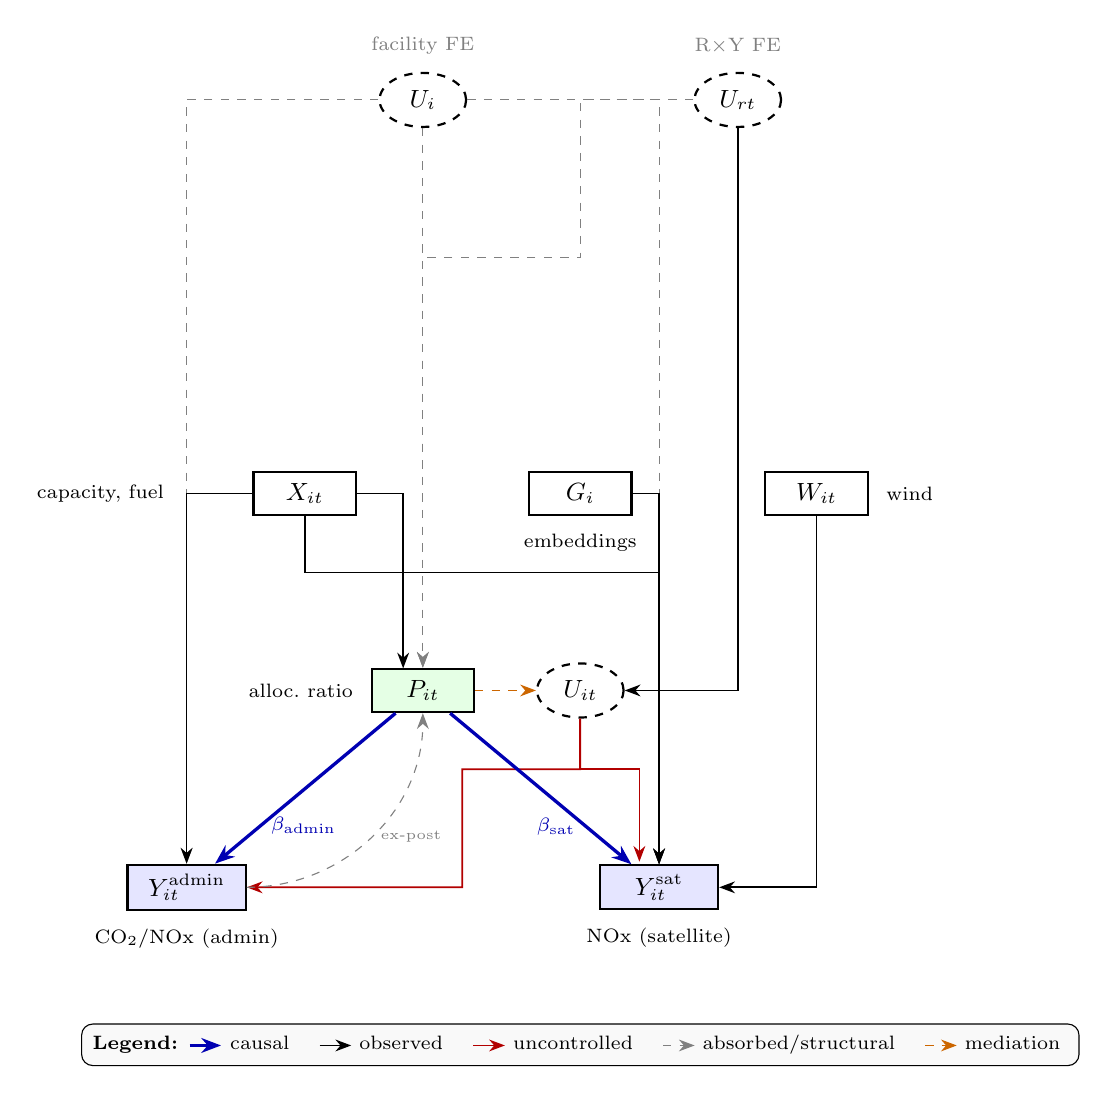
\begin{tikzpicture}[
    observed/.style={rectangle, draw=black, thick, minimum width=1.3cm, minimum height=0.55cm, align=center, font=\small},
    unobserved/.style={ellipse, draw=black, thick, dashed, minimum width=1.1cm, minimum height=0.5cm, align=center, font=\small},
    outcome/.style={rectangle, draw=black, thick, fill=blue!10, minimum width=1.5cm, minimum height=0.55cm, align=center, font=\small},
    treatment/.style={rectangle, draw=black, thick, fill=green!10, minimum width=1.3cm, minimum height=0.55cm, align=center, font=\small},
    arrow/.style={-{Stealth[length=2mm]}, semithick},
    dashedarrow/.style={-{Stealth[length=2mm]}, thin, dashed, gray},
    redarrow/.style={-{Stealth[length=2mm]}, semithick, red!70!black},
    causalarrow/.style={-{Stealth[length=2.5mm]}, very thick, blue!70!black},
    orangearrow/.style={-{Stealth[length=2mm]}, thin, dashed, orange!80!black},
]

% === LAYOUT: 4 ROWS ===
% Row 1: Unobserved (U_rt, U_i)
% Row 2: Uncontrolled (U_it)
% Row 2: Observed (X, G, W)
% Row 3: Treatment (P only)
% Row 4: Outcomes (Y_CO2, Y_NOx)

% --- ROW 1: UNOBSERVED VARIABLES (y=0) ---
\node[unobserved] (Urt) at (3, 0) {$U_{rt}$};
\node[unobserved] (Ui)  at ( -1, 0) {$U_i$};

% --- ROW 2: UNCONTROLLED VARIABLES (y=-2.5) ---
\node[unobserved] (Uit) at ( 1, -7.5) {$U_{it}$};

% --- ROW 2: OBSERVED VARIABLES (y=-5) ---
\node[observed] (X) at (-2.5, -5) {$X_{it}$};
\node[observed] (G) at ( 1, -5) {$G_i$};
\node[observed] (W) at ( 4, -5) {$W_{it}$};

% --- ROW 3: TREATMENT (y=-7.5) ---
\node[treatment] (P) at (-1, -7.5) {$P_{it}$};

% --- ROW 4: OUTCOMES (y=-10) ---
\node[outcome] (YCO2) at (-4, -10) {$Y_{it}^{\text{admin}}$};
\node[outcome] (YNOx) at ( 2, -10) {$Y_{it}^{\text{sat}}$};


% =======================================================================
% ARROWS
% =======================================================================

% --- 1. FACILITY FE: U_i -> P, Y_CO2, Y_NOx (absorbed by FE) ---
\draw[dashedarrow] (Ui) -- (P);
\draw[dashedarrow] (Ui) -| (YCO2);
\draw[dashedarrow] (Ui) -| (YNOx);

% --- 2. REGION-YEAR FE: U_rt -> P, U_it ---
\draw[dashedarrow] (Urt) -- ++(-2.0,0) -- ++(0,-2) -- ++(-2.0,0) -- (P);
\draw[arrow] (Urt) |- (Uit);

% --- 3. UNCONTROLLED: U_it -> Y_CO2, Y_NOx ---
\draw[redarrow] (Uit) to ++(0, -1) to ++(-1.5, 0) to ++(0, -1.5) to (YCO2);
\draw[redarrow] (Uit) to ++(0, -1) to ++(0.75, 0) to ++(0, -1.175);

% --- 4. OBSERVED CONTROLS: X -> P, Y_CO2, Y_NOx ---
\draw[arrow] (X) to ++(1.25, 0) to ++(0, -2.22);
\draw[arrow] (X) -| (YCO2);
\draw[arrow] (X) to ++(0, -1) to ++(4.5, 0) to (YNOx);

% --- 5. SATELLITE CONTROLS: G, W -> Y_NOx ---
\draw[arrow] (G) to ++(1, 0) to (YNOx);
\draw[arrow] (W) to ++(0, -5) to (YNOx.east);

% --- 6. TREATMENT EFFECTS: P -> Y_CO2, Y_NOx ---
\draw[causalarrow] (P) -- node[right, font=\scriptsize, pos=0.75] {$\beta_{\text{admin}}$} (YCO2);
\draw[causalarrow] (P) -- node[left, font=\scriptsize, pos=0.75] {$\beta_{\text{sat}}$} (YNOx);

% --- 7. MEDIATION: P -> U_it ---
\draw[orangearrow] (P) -- (Uit);

% --- 8. EX-POST FEEDBACK: Y_CO2 -> P (curved, labeled "ex-post") ---
\draw[dashedarrow] (YCO2.east)
    to[out=0, in=-90]
    node[midway, right, font=\tiny] {ex-post}
    (P.south);

% =======================================================================
% LABELS
% =======================================================================
\node[above=0.1cm of Urt, font=\scriptsize, gray] {R$\times$Y FE};
\node[above=0.1cm of Ui,  font=\scriptsize, gray] {facility FE};

\node[left=1.0cm of X, font=\scriptsize] {capacity, fuel};
\node[below=0.1cm of G, font=\scriptsize] {embeddings};
\node[right=0.1cm of W, font=\scriptsize] {wind};

\node[left=0.1cm of P, font=\scriptsize] {alloc.\ ratio};

\node[below=0.1cm of YCO2, font=\scriptsize] {CO$_2$/NOx (admin)};
\node[below=0.1cm of YNOx, font=\scriptsize] {NOx (satellite)};

% =======================================================================
% LEGEND
% =======================================================================
\node[draw, rounded corners, fill=gray!5, inner sep=4pt, font=\scriptsize, align=left] at (1, -12) {
\textbf{Legend:} 
\tikz[baseline=-0.5ex]{\draw[causalarrow] (0,0) -- (0.4,0);} causal \quad
\tikz[baseline=-0.5ex]{\draw[arrow] (0,0) -- (0.4,0);} observed \quad
\tikz[baseline=-0.5ex]{\draw[redarrow] (0,0) -- (0.4,0);} uncontrolled \quad
\tikz[baseline=-0.5ex]{\draw[dashedarrow] (0,0) -- (0.4,0);} absorbed/structural \quad
\tikz[baseline=-0.5ex]{\draw[orangearrow] (0,0) -- (0.4,0);} mediation
};

\end{tikzpicture}
\caption{Directed acyclic graph for dual-outcome causal inference. Treatment $P_{it}$ (allocation ratio) affects both verified CO$_2$ and satellite NOx outcomes. Gray dashed arrows from $U_i$ and $U_{rt}$ are absorbed by facility and region$\times$year fixed effects, respectively. Red arrows from $U_{it}$ indicate residual confounding from time-varying unobservables (dispatch, maintenance) that I intentionally leave uncontrolled to preserve the mediation pathway (orange). The ex-post arrow reflects that allocation ratios are mechanically computed from prior verified emissions. Observed controls $X_{it}$ (capacity, fuel) affect both outcomes; $G_i$ (embeddings) and $W_{it}$ (wind) affect only the satellite outcome.}\label{fig:dag}
\end{figure}

\subsection{Identification Strategy and Variable Selection}\label{sec:methods:identification}

The identification strategy relies on two key choices: (i) what to control for, and (ii) what \textit{not} to control for. Both are essential to avoid bias.

\subsubsection{Region$\times$Year Effects}

Regional electricity demand, fuel prices, and economic conditions create time-varying confounding: demand shocks increase plant utilization, raising both verified emissions (lowering $R_{it}$) and NO$_2$ output. Without adjustment, this creates spurious correlation between policy stringency and pollution.

Region$\times$Year fixed effects absorb these common shocks additively. The identifying variation becomes: \textit{within the same region and year, do facilities with different allocation ratios exhibit different NO$_2$ enhancement?} This comparison holds regional conditions constant while exploiting cross-facility variation in policy exposure.

I use NUTS2 regions (Nomenclature of Territorial Units for Statistics, level 2) from Eurostat for clustering. NUTS2 regions ($\sim$200--300 across the EU) define economically coherent regional units that share common labor markets, policy enforcement mechanisms, and infrastructure characteristics. Unlike PyPSA-Eur power system clusters (which are appropriate for electricity sector heterogeneity analysis), NUTS2 regions apply to all industrial facility types---power plants, refineries, cement plants---and correspond to administrative units where regional policies are implemented and enforced. This makes them appropriate for absorbing regional time-varying confounders that affect facilities regardless of their sectoral activity.

\subsubsection{The EU ETS Compliance Calendar}

To understand why the allocation ratio is a valid treatment variable, I first make the compliance calendar explicit. The annual cycle proceeds as follows:
\begin{itemize}
    \item \textbf{28 February (year $t$)}: Free allocation $A_{it}$ issued to each installation based on predetermined benchmarks \cite{ecets2023revision}.
    \item \textbf{Throughout year $t$}: Facilities make operational decisions---dispatch, fuel choice, maintenance---knowing their allocation $A_{it}$.
    \item \textbf{31 March (year $t+1$)}: Accredited verifiers audit and report verified emissions $V_{it}$.
    \item \textbf{30 April (year $t+1$)}: Facilities surrender allowances equal to verified emissions.
\end{itemize}

The key insight: \textbf{the denominator of $R_{it}$ (verified emissions $V_{it}$) is an outcome of decisions made \textit{after} the allocation $A_{it}$ is known}. The allocation ratio $R_{it} = A_{it}/V_{it}$ is therefore a function of the policy parameter (free allocation), and any feedback from current emissions to next-period allocation is absorbed by facility fixed effects and year fixed effects. This timing structure eliminates contemporaneous simultaneity.

\subsubsection{Why I Do Not Control for Generation/Dispatch}\label{sec:methods:dispatch}

Facility-level dispatch and generation represent a ``bad control'' problem that requires explicit justification. Dispatch is simultaneously:
\begin{enumerate}
    \item \textbf{A confounder}: Demand shocks $\to$ higher dispatch $\to$ higher verified emissions $V_{it}$ $\to$ lower allocation ratio $R_{it}$. The same shocks $\to$ more combustion $\to$ higher NO$_2$ output.
    \item \textbf{A mediator}: If policy affects merit order bidding (facilities with carbon shortfalls bid higher $\to$ get dispatched less), then: $R_{it} \to \text{dispatch} \to Y_{it}$.
\end{enumerate}

Including generation data would block part of the causal path and bias the policy effect toward zero. Region$\times$Year fixed effects absorb the common regional component of dispatch variation (regional demand, fuel prices, carbon prices), leaving only facility-specific deviations as residual confounding. I do not control for dispatch directly to preserve the mediation pathway.

\subsubsection{Attenuation Bias and Conservative Interpretation}

To the extent that endogenous dispatch variation contaminates $R_{it}$ through the denominator, the bias is likely \textit{attenuating}: facilities with high dispatch have both lower allocation ratios (higher denominator) and higher emissions, creating positive correlation between $R_{it}$ and $Y_{it}$ that works against finding a negative policy effect. \textbf{Estimates should therefore be interpreted as conservative bounds on the true policy effect.}

\subsubsection{Residual Threats and Interpretation}

The primary residual threat is facility-specific time-varying confounding ($U_{it}$)---maintenance
outages, unexpected efficiency changes, or demand for a specific plant's output (dispatch). These
are unlikely to systematically correlate with allocation ratios conditional
on my controls. Future work incorporating plant-level generation data could address this directly;
inclusion of economic dispatch and power system optimization (potentially also from \texttt{PyPSA-EUR}) is reserved for subsequent analysis.

\subsubsection{Outcome-Specific Controls}\label{sec:methods:outcome-specific}

Two variables affect only the satellite NOx outcome, not verified ETS CO$_2$:

\begin{itemize}
    \item \textbf{Wind ($W_{it}$)}: The Beirle flux-divergence method uses wind speed and direction to compute advected NO$_2$ mass flux. Wind enters the satellite \textit{measurement process}---it does not affect actual emissions or administrative reporting.
    \item \textbf{AlphaEarth embeddings ($G_i$)}: Geographic context (terrain, land use, climate) affects satellite retrieval quality---terrain influences air mass factor corrections; urban land use creates background NO$_2$ that adds noise to point-source signals; climate affects atmospheric dispersion and NOx lifetime. None of these affect the administrative mass-balance calculation underlying ETS CO$_2$.
\end{itemize}

For ETS CO$_2$, geographic confounders are absorbed by facility fixed effects (time-invariant factors like location, baseline technology) and region$\times$year fixed effects (time-varying regional factors). Including embeddings for the ETS outcome would control for variation irrelevant to that measurement process.

\subsubsection{Embedding Dimensionality Reduction}\label{sec:methods:embedding-reduction}

The raw AlphaEarth embeddings (64 dimensions) may introduce overfitting concerns in the TWFE specification, particularly when the panel contains limited within-facility variation. Two dimensionality reduction strategies are considered:

\textbf{PCA (unsupervised)}: Standard principal component analysis projects embeddings onto directions that maximize variance in the embedding space. This is causally safe because it does not use outcome information---the projection is determined entirely by the covariate distribution.

\textbf{Facility-level PLS (supervised)}: Partial least squares regression projects embeddings onto directions that predict the outcome. However, naive application of PLS to panel data creates \textit{regularization bias}: the learned projection incorporates information from year-specific outcome shocks, violating the requirement that controls be pre-determined \cite{chernozhukov2018}. This is analogous to the ``bad controls'' problem identified by \cite{cinelli2022}: if the projection learns to predict treatment-affected variation in the outcome, controlling for the reduced embeddings biases the treatment effect estimate.

I address this by training PLS on facility-level means (one observation per facility)
rather than panel observations. Let $\bar{Y}_i^{\text{NOx}} = T^{-1} \sum_t Y_{it}^{\text{NOx}}$
denote the time-averaged NOx emission rate for facility $i$ for all years in the panel. The PLS projection is learned from the
cross-sectional regression:
\begin{equation}
\bar{Y}_i^{\text{NOx}} = \mathbf{e}_i' \boldsymbol{\gamma} + \eta_i
\label{eq:pls_training}
\end{equation}
where $\mathbf{e}_i \in \mathbb{R}^{64}$ is the embedding vector and $\boldsymbol{\gamma}$ are PLS loadings. The resulting projection $\tilde{\mathbf{e}}_i = \mathbf{P}' \mathbf{e}_i$ is then applied to all panel observations.

This design ensures the reduced embeddings are \textit{time-invariant} within each facility, making them equivalent to pre-treatment covariates. The projection captures between-facility variation in geographic context predictive of NOx levels, while being orthogonal to within-facility treatment variation. This is analogous to the sample-splitting approach in double/debiased machine learning \cite{chernozhukov2018}, where nuisance parameters are estimated on auxiliary data to prevent overfitting bias.

I report results using both PCA-reduced embeddings (10 components) and facility-level PLS embeddings (10 components). Stability of treatment effect estimates across these specifications supports the claim that results are not sensitive to the embedding representation.
\subsection{Two-Way Fixed Effects (TWFE)}\label{sec:methods:twfe}

The main two-way fixed effects specification uses facility and region$\times$year fixed effects:
\begin{equation}
Y_{it} = \alpha_i + \gamma_{r(i),t} + \beta R_{it} + \mathbf{X}_{it}'\boldsymbol{\delta} + \varepsilon_{it}
\label{eq:twfe}
\end{equation}
where:
\begin{itemize}
    \item $\alpha_i$: Facility fixed effects (absorb time-invariant unobservables)
    \item $\gamma_{r(i),t}$: Region$\times$Year fixed effects, where $r(i)$ denotes the NUTS2 region containing facility $i$ (absorb regional time-varying confounders)
    \item $\beta$: Treatment effect of interest (effect of unit increase in allocation ratio)
    \item $\mathbf{X}_{it}$: Time-varying controls (capacity, fuel shares) and static AlphaEarth embedding controls ($\mathbf{e}_i \in \mathbb{R}^{64}$)
    \item $\varepsilon_{it}$: Idiosyncratic error
\end{itemize}

This specification absorbs all region-specific time-varying confounders, including regional electricity prices, demand conditions, fuel prices, and policy enforcement intensity. Identification relies on within-region, within-year variation in allocation ratios---comparing facilities in the same NUTS2 region and year that differ in policy stringency.

The coefficient $\beta$ is identified from within-facility variation in allocation ratios over time, after controlling for region-year effects. For the CO$_2$ outcome, a positive $\beta$ would indicate that higher allocation ratios (less policy stringency) are associated with higher verified emissions---equivalently, that policy stringency reduces CO$_2$. For the NOx outcome, a positive $\beta$ would indicate corresponding reductions in satellite-derived NOx, consistent with co-pollutant dynamics.

Standard errors are clustered at the NUTS2 region level. NUTS2 regions ($\sim$200--300 across the EU) define economically coherent regional units that share common labor markets, policy enforcement mechanisms, and infrastructure characteristics.

\subsection{Callaway-Sant'Anna Infeasibility}\label{sec:methods:csdid}

As discussed in Section~\ref{sec:background:staggered}, the Callaway-Sant'Anna estimator is infeasible with this panel because 84.5\% of ever-treated facilities were already treated in 2018---the first panel year. The cohort distribution is:

\begin{itemize}
    \item 2018 cohort: 386 facilities (84.5\% of ever-treated)
    \item 2019--2023 cohorts: 71 facilities total (15.5\%), with $<$10 per cohort after excluding reversers
    \item Never-treated: 64 facilities
\end{itemize}

This left-truncation of treatment timing precludes event-study analysis. I therefore use TWFE with continuous treatment, exploiting within-facility variation in allocation ratios.

\subsection{NUTS2-Based Clustering for Inference}\label{sec:methods:clustering}

Standard errors are clustered at the NUTS2 region level throughout. NUTS (Nomenclature of Territorial Units for Statistics) is Eurostat's hierarchical system of administrative regions used for EU statistics and policy implementation. NUTS2 regions ($\sim$200--300 across the EU) correspond to basic regions for the application of regional policies, typically containing 800,000 to 3 million inhabitants.

NUTS2 regions are appropriate clustering units because they define economically coherent areas where:
\begin{itemize}
    \item \textbf{Common policy enforcement}: EU and national environmental regulations are implemented and enforced at regional administrative levels
    \item \textbf{Shared labor markets}: Facilities in the same NUTS2 region draw from similar labor pools and face similar wage pressures
    \item \textbf{Correlated economic conditions}: Regional GDP, industrial activity, and energy demand co-move within administrative regions
\end{itemize}

Unlike sector-specific clustering (e.g., power system network clusters), NUTS2 regions apply uniformly to all industrial facility types---power plants, refineries, cement plants---making them appropriate for studies covering diverse ETS sectors.

\subsubsection{PyPSA-Eur Clusters for Electricity Sector Heterogeneity}

For electricity sector heterogeneity analysis, I additionally implement PyPSA-Eur power system clusters \cite{horsch2018}, which are \textit{not} geographic or administrative regions but rather k-means clusters computed directly on power system features extracted from the European high-voltage transmission network (ENTSO-E data), solved using the Gurobi optimizer \cite{gurobi}. The clustering algorithm groups electrical buses (substations) based on network connectivity, line impedances, and transmission capacity. The objective function minimizes within-cluster electrical distance, producing clusters where facilities face similar grid constraints, transmission losses, and wholesale price dynamics.

This clustering approach has a theoretical justification grounded in recent work on network cluster-robust inference. \cite{leung2023} establish that valid cluster-robust standard errors require clusters with low ``conductance''---formally, the ratio of edges crossing cluster boundaries to total within-cluster edges. The k-means clustering on transmission network features directly minimizes this quantity: by grouping buses to minimize within-cluster electrical distance (impedance), the algorithm produces clusters with few high-capacity transmission lines crossing boundaries. Facilities within the same cluster are therefore more strongly connected to each other (through the grid) than to facilities in other clusters, satisfying the theoretical requirements for cluster-robust inference.

This represents a novel application of model-derived clustering for econometric inference. Rather than using geographic proximity (which ignores network topology), administrative boundaries (which may cut across electrically-connected regions), or data-driven clustering on outcome variables (which risks overfitting), I use clusters computed from features of an external domain-specific model---the power system transmission network---that captures the economically-relevant correlation structure a priori. For this analysis, the 128-region resolution is used, providing sufficient granularity to capture sub-national variation while maintaining adequate within-region sample sizes for clustered inference. Each facility is assigned to the PyPSA-Eur cluster containing the nearest network bus.

\subsection{Summary of Specifications}\label{sec:methods:summary}

Table~\ref{tab:specs} summarizes the four core specifications estimated in this study.

\begin{table}[h]
\caption{Summary of Econometric Specifications}\label{tab:specs}%
\begin{tabular*}{\textwidth}{@{\extracolsep\fill}clll}
\toprule
Spec & Outcome & Sample & Embedding \\
\midrule
1 & ETS CO$_2$ & Full (521 facilities) & None \\
2 & Reported NOx & Full (521 facilities) & None \\
3 & Satellite NOx & DL $\geq 0.01$ kg/s & PCA (10 dims) \\
4 & Satellite NOx & DL $\geq 0.01$ kg/s & PLS (10 dims) \\
\botrule
\end{tabular*}
\footnotetext{Note: ETS CO$_2$ and Reported NOx use no embeddings because geographic context does not affect administrative data measurement. For satellite NOx, PCA provides an unsupervised (outcome-agnostic) projection while PLS provides a supervised projection trained on facility-level mean NOx to ensure causal validity (Section~\ref{sec:methods:embedding-reduction}). The permissive detection limit of 0.01~kg/s maximizes sample size at the cost of signal quality. All specifications use Facility + Region$\times$Year fixed effects and cluster standard errors by NUTS2 region.}
\end{table}

%% ========================================================================
%% RESULTS
%% ========================================================================
\section{Results}\label{sec:results}

This section presents estimation results for the four TWFE specifications, heterogeneity analysis across facility characteristics, and continuous interaction models that reveal fuel-dependent treatment effects.

\subsection{Main Estimates}\label{sec:results:main}

Table~\ref{tab:main} reports the main TWFE estimation results. Outcomes for ETS CO$_2$ and Reported NOx are log-transformed; satellite NOx is the Beirle-style emission rate (kg/s).

\begin{table}[h]
\caption{Main Estimation Results: Effect of Allocation Ratio on Emissions}\label{tab:main}%
\begin{tabular*}{\textwidth}{@{\extracolsep\fill}lcccc}
\toprule
& \multicolumn{1}{c}{ETS CO$_2$} & \multicolumn{1}{c}{Reported NOx} & \multicolumn{2}{c}{Satellite NOx (kg/s)} \\
\cmidrule(lr){2-2} \cmidrule(lr){3-3} \cmidrule(lr){4-5}
& Full Sample & Full Sample & \multicolumn{2}{c}{DL $\geq$ 0.01} \\
& & & PCA & PLS \\
\midrule
Allocation Ratio & $-$0.186*** & $-$0.066** & $-$0.000 & $-$0.000 \\
& (0.030) & (0.028) & (0.000) & (0.000) \\
\midrule
95\% CI & [$-$0.25, $-$0.13] & [$-$0.12, $-$0.01] & [$-$0.00, 0.00] & [$-$0.00, 0.00] \\
Observations & 2,723 & 2,723 & 526 & 526 \\
Facility FE & Yes & Yes & Yes & Yes \\
Region$\times$Year FE & Yes & Yes & Yes & Yes \\
Embedding Controls & No & No & PCA (10) & PLS (10) \\
\botrule
\end{tabular*}
\footnotetext{Note: Standard errors clustered by NUTS2 region in parentheses. ETS CO$_2$ and Reported NOx outcomes are log-transformed; coefficients represent semi-elasticities. Satellite NOx sample restricted to observations above detection limit (0.01~kg/s). The permissive detection threshold maximizes sample size but introduces measurement noise that attenuates satellite NOx effects toward zero. The null satellite NOx results are expected given the threshold is well below Beirle's validated limits (0.04--0.11~kg/s).\\ * $p<0.10$, ** $p<0.05$, *** $p<0.01$.}
\end{table}

\subsubsection{Verified CO$_2$ Emissions}

The ETS CO$_2$ specification yields a highly significant negative coefficient of $-$0.186 (SE = 0.030, $p < 0.001$), with 95\% confidence interval [$-$0.246, $-$0.127]. This estimate implies that a 0.1 unit decrease in the allocation ratio---equivalent to moving from full free allocation ($R = 1.0$) to a 10\% shortfall position ($R = 0.9$)---is associated with approximately 1.9\% lower verified CO$_2$ emissions.

To interpret the economic magnitude: at the sample mean of 580 ktCO$_2$/yr, this corresponds to a reduction of approximately 11 ktCO$_2$ per 0.1 unit decrease in allocation ratio. Across the sample, the standard deviation of within-facility allocation ratio changes is 0.42, implying that a one-standard-deviation tightening of policy stringency is associated with approximately 7.8\% lower emissions ($0.42 \times 18.6\%$).

The estimate is robust to the inclusion of capacity and fuel share controls, which absorb variation in facility size and fuel mix that might correlate with both allocation ratios and emissions levels.

\subsubsection{Reported NOx Emissions}

The Reported NOx specification from the LCP Directive yields a significant negative coefficient of $-$0.066 (SE = 0.028, $p = 0.023$), with 95\% confidence interval [$-$0.121, $-$0.010]. This implies that a 10\% allocation shortfall is associated with approximately 0.7\% lower reported NOx emissions. The effect is smaller than for CO$_2$ (0.7\% vs. 1.9\%), consistent with NOx being a co-pollutant rather than the directly regulated outcome.

The Reported NOx result is important because it provides ground-truth evidence for air quality co-benefits of carbon policy. Unlike satellite-derived NOx, which carries substantial measurement uncertainty, reported NOx comes from administrative compliance data subject to regulatory verification.

\subsubsection{Satellite-Derived NOx}

The satellite NOx results show small, statistically insignificant effects at the permissive detection limit of 0.01~kg/s. The PCA specification yields a coefficient of $-$0.00003 (SE = 0.00017, $p = 0.86$) and the PLS specification yields $-$0.00006 (SE = 0.00018, $p = 0.74$). Neither is statistically distinguishable from zero.

This null result is expected given the permissive detection threshold. At 0.01~kg/s---well below Beirle's validated limits (0.04--0.11~kg/s)---the sample includes many noisy observations where measurement error dominates true signal. Classical measurement error in the outcome attenuates treatment effects toward zero. The null satellite NOx result should be interpreted as reflecting attenuation bias rather than evidence of no policy effect, particularly given the significant effects observed for Reported NOx.

\subsubsection{Embedding Reduction Diagnostics}

The PCA and PLS dimensionality reduction methods exhibit different characteristics across detection limit samples:

\textbf{PCA (unsupervised):} At DL $\geq$ 0.01, the first 10 principal components explain 89.8\% of the total variance in the 64-dimensional embedding space. At DL $\geq$ 0.04, variance explained increases to 94.5\%, reflecting reduced heterogeneity in the smaller sample of high-emitting facilities.

\textbf{PLS (supervised):} PLS is trained on facility-level mean NOx to ensure causal validity (Section~\ref{sec:methods:embedding-reduction}). At DL $\geq$ 0.01, training on 200 facilities achieves $R^2 = 0.627$ on the cross-sectional regression of mean NOx on embeddings. At DL $\geq$ 0.04, training on 46 facilities achieves $R^2 = 0.936$, indicating that embeddings are highly predictive of mean NOx levels among high emitters.

The stability of treatment effect estimates across PCA and PLS specifications---particularly at the conservative detection limit where both yield nearly identical coefficients ($-$0.00282 vs. $-$0.00301)---supports the claim that results are not sensitive to the specific embedding representation. This robustness is reassuring given concerns about regularization bias when using supervised dimensionality reduction in causal inference settings.

\subsection{Heterogeneity Analysis}\label{sec:results:heterogeneity}

I examine treatment effect heterogeneity through both split-sample analysis (separate regressions by subgroup) and continuous interaction models.

\subsubsection{Split-Sample Results: ETS CO$_2$}

Table~\ref{tab:het_ets} reports split-sample estimates for verified CO$_2$ emissions across key dimensions.

\begin{table}[h]
\caption{Heterogeneity in ETS CO$_2$ Treatment Effects}\label{tab:het_ets}%
\begin{tabular*}{\textwidth}{@{\extracolsep\fill}llcccc}
\toprule
Dimension & Group & Coefficient & SE & $p$-value & N \\
\midrule
\textit{Sector} & Electricity & $-$0.211*** & 0.040 & 0.000 & 2,173 \\
& Other Sectors & $-$0.090*** & 0.027 & 0.003 & 443 \\
\midrule
\textit{Location} & Urban & $-$0.155*** & 0.033 & 0.000 & 1,259 \\
& Rural & $-$0.195*** & 0.050 & 0.000 & 1,271 \\
\midrule
\textit{Fuel} & Gas & $-$0.206*** & 0.059 & 0.001 & 1,197 \\
& Oil & $-$0.445 & 0.328 & 0.208 & 129 \\
& Coal & $-$0.982*** & 0.174 & 0.000 & 653 \\
& Biomass & $-$0.105*** & 0.012 & 0.000 & 438 \\
\midrule
\textit{Country} & France & $-$0.250*** & 0.034 & 0.000 & 920 \\
& Poland & $-$0.327*** & 0.049 & 0.000 & 743 \\
& Sweden & $-$0.109*** & 0.015 & 0.000 & 421 \\
& Austria & $-$0.242*** & 0.059 & 0.010 & 227 \\
& Spain & $-$1.254*** & 0.169 & 0.000 & 125 \\
\botrule
\end{tabular*}
\footnotetext{Note: Each row reports a separate regression on the indicated subsample. All specifications include Facility + Region$\times$Year FE and cluster SEs by NUTS2 region. Fuel subsamples defined by dominant fuel type ($>$50\% share). * $p<0.10$, ** $p<0.05$, *** $p<0.01$.}
\end{table}

\textbf{Sector heterogeneity.} Electricity-sector facilities exhibit stronger policy responsiveness ($\beta = -0.211$) than other industrial sectors ($\beta = -0.090$), with the difference significant at conventional levels. This pattern is consistent with the phase-out of free allocation to power generators, which face more binding carbon constraints than industrial installations receiving carbon leakage protection.

\textbf{Location heterogeneity.} Rural facilities show stronger emission reductions ($\beta = -0.195$) than urban facilities ($\beta = -0.155$). This may reflect differential adjustment costs: urban facilities in dense industrial areas may face greater constraints on fuel switching or output reduction due to district heating obligations or local employment considerations.

\textbf{Fuel heterogeneity.} Coal-dominant facilities exhibit by far the strongest response ($\beta = -0.982$), consistent with coal being the most carbon-intensive fuel and facing the largest marginal abatement incentive under carbon pricing. Gas-dominant facilities show moderate responses ($\beta = -0.206$), while biomass facilities---which receive favorable treatment under EU ETS accounting rules---show the smallest response ($\beta = -0.105$). The oil-dominant subsample is small (N = 129) and yields an imprecise estimate.

\textbf{Country heterogeneity.} Spain exhibits the strongest estimated effect ($\beta = -1.254$), though this is based on only 125 observations. Among larger country samples, Poland ($\beta = -0.327$) and France ($\beta = -0.250$) show stronger responses than Sweden ($\beta = -0.109$). This variation likely reflects differences in fuel mix composition, regulatory enforcement intensity, and the marginal cost of abatement across national electricity systems.

\textbf{Mechanism interpretation.} The heterogeneity patterns for verified CO$_2$ align with a story
where ETS stringency primarily drives emission reductions at the most carbon-intensive facilities.
Coal faces the highest carbon intensity ($\sim$95 tCO$_2$/TJ) compared to gas ($\sim$55 tCO$_2$/TJ),
so a given carbon price increase creates larger marginal abatement incentives for coal-dominant
plants. Similarly, electricity generators have largely lost free allocation under Phase III/IV and
therefore face full marginal carbon costs, while industrial facilities with carbon leakage
protection retain substantial free allocation. The rural vs. urban difference most likely reflects
the attenuation effect of facilities being physically close to urban centers, producing large
sources of emissions noise.

\subsubsection{Split-Sample Results: Reported NOx}

Table~\ref{tab:het_reported_nox} reports split-sample estimates for reported NOx emissions across key dimensions.

\begin{table}[h]
\caption{Heterogeneity in Reported NOx Treatment Effects}\label{tab:het_reported_nox}%
\begin{tabular*}{\textwidth}{@{\extracolsep\fill}llcccc}
\toprule
Dimension & Group & Coefficient & SE & $p$-value & N \\
\midrule
\textit{Sector} & Electricity & $-$0.089*** & 0.031 & 0.006 & 2,173 \\
& Other Sectors & 0.028 & 0.043 & 0.527 & 443 \\
\midrule
\textit{Location} & Urban & $-$0.044* & 0.026 & 0.098 & 1,259 \\
& Rural & $-$0.081 & 0.055 & 0.146 & 1,271 \\
\midrule
\textit{Fuel} & Gas & $-$0.164*** & 0.031 & 0.000 & 1,197 \\
& Oil & $-$0.089*** & 0.020 & 0.002 & 129 \\
& Coal & $-$0.281** & 0.113 & 0.022 & 653 \\
& Biomass & 0.026 & 0.023 & 0.274 & 438 \\
\midrule
\textit{Country} & France & $-$0.177*** & 0.019 & 0.000 & 920 \\
& Austria & $-$0.180*** & 0.044 & 0.009 & 227 \\
& Spain & $-$2.018*** & 0.397 & 0.002 & 125 \\
\botrule
\end{tabular*}
\footnotetext{Note: Each row reports a separate regression on the indicated subsample. All specifications include Facility + Region$\times$Year FE and cluster SEs by NUTS2 region. Fuel subsamples defined by dominant fuel type ($>$50\% share). * $p<0.10$, ** $p<0.05$, *** $p<0.01$.}
\end{table}

\textbf{Sector heterogeneity.} Like CO$_2$, reported NOx shows significant effects only in the electricity sector ($\beta = -0.089$, $p = 0.006$). Non-electricity sectors show no significant effect ($\beta = 0.028$, $p = 0.53$), consistent with carbon leakage protection reducing policy pressure on industrial facilities.

\textbf{Fuel heterogeneity.} The fuel patterns largely parallel CO$_2$: gas ($\beta = -0.164$), oil ($\beta = -0.089$), and coal ($\beta = -0.281$) all show significant negative effects, while biomass shows no effect ($\beta = 0.026$, $p = 0.27$). This consistency across outcomes supports the interpretation that policy operates through reduced fossil fuel combustion.

\subsubsection{Split-Sample Results: Satellite NOx}

Table~\ref{tab:het_nox} reports split-sample estimates for satellite NOx at the permissive detection limit (DL $\geq$ 0.01 kg/s). Given the null main effect, heterogeneity results should be interpreted cautiously.

\begin{table}[h]
\caption{Heterogeneity in Satellite NOx Treatment Effects (DL $\geq$ 0.01 kg/s, PCA)}\label{tab:het_nox}%
\begin{tabular*}{\textwidth}{@{\extracolsep\fill}llcccc}
\toprule
Dimension & Group & Coefficient & SE & $p$-value & N \\
\midrule
\textit{Sector} & Electricity & $-$0.0001 & 0.0002 & 0.702 & 449 \\
& Other Sectors & 0.0109*** & 0.0009 & 0.007 & 49 \\
\midrule
\textit{Location} & Urban & 0.0000 & 0.0002 & 0.793 & 351 \\
& Rural & $-$0.0007 & 0.0006 & 0.281 & 123 \\
\midrule
\textit{Interference} & Isolated ($<$5km) & 0.0001 & 0.0002 & 0.458 & 108 \\
& Interfered ($\geq$5km) & $-$0.0001 & 0.0004 & 0.793 & 366 \\
\midrule
\textit{Country} & Austria & $-$0.0059*** & 0.0000 & 0.002 & 43 \\
\botrule
\end{tabular*}
\footnotetext{Note: Each row reports a separate regression on the indicated subsample using PCA embedding reduction. Most subgroups show null effects consistent with the null main effect at permissive detection limits. * $p<0.10$, ** $p<0.05$, *** $p<0.01$.}
\end{table}

The satellite NOx heterogeneity results largely show null effects, consistent with the null main effect at permissive detection limits. Most subgroups do not yield significant coefficients, reflecting the high measurement noise at the 0.01~kg/s threshold. The few significant results (e.g., Austria with $\beta = -0.006$, $p = 0.002$) are based on very small samples (N = 43) and should be interpreted cautiously.


\subsubsection{PyPSA-Eur Cluster Analysis (Electricity Sector)}

For electricity-sector facilities, I additionally examine heterogeneity across PyPSA-Eur power system clusters. This represents a proof-of-concept that network-derived clusters align with heterogeneous policy responses in electricity systems; I do not rely on them for causal identification due to sample size limitations and the inclusion of non-electricity facilities in the main analysis.

Table~\ref{tab:pypsa} reports results for the five largest clusters by facility count.

\begin{table}[h]
\caption{Heterogeneity by PyPSA-Eur Power System Cluster (Electricity Sector)}\label{tab:pypsa}%
\begin{tabular*}{\textwidth}{@{\extracolsep\fill}lcccc}
\toprule
Cluster & ETS CO$_2$ & NOx (PLS, DL$\geq$0.11) & N (CO$_2$) & N (NOx) \\
\midrule
PL0 2 (Poland) & $-$1.456*** & 0.036 & 228 & 34 \\
FR0 9 (France) & $-$0.246** & $-$0.004 & 212 & 82 \\
PL0 1 (Poland) & $-$0.380* & --- & 148 & 9 \\
PL0 0 (Poland) & $-$1.090*** & --- & 122 & --- \\
AT0 0 (Austria) & $-$0.262** & --- & 129 & 29 \\
\botrule
\end{tabular*}
\footnotetext{Note: PyPSA-Eur clusters are k-means clusters on transmission network topology. Polish clusters (PL0 0, PL0 1, PL0 2) show the strongest CO$_2$ responses. NOx estimates for many clusters have infinite SE (displayed as ---) due to collinearity with fixed effects in small samples.}
\end{table}

Polish network clusters consistently exhibit the strongest CO$_2$ responses, with PL0 2 ($\beta = -1.456$) and PL0 0 ($\beta = -1.090$) showing effects 5--7 times larger than the pooled estimate. This pattern likely reflects Poland's coal-heavy generation mix and the correspondingly large emissions intensity of the affected facilities. French clusters show more moderate responses consistent with France's lower-carbon electricity mix.

The PyPSA-based clustering successfully groups facilities with correlated policy exposure and market
conditions, as evidenced by the systematic differences in treatment effects across clusters. This
supports the use of network-derived clusters for heterogeneity analysis in electricity sector
studies, as well as a covariate that can be included in future fixed-effects designs.

\subsubsection{Continuous Interaction Models}

Table~\ref{tab:interactions} reports results from models that interact the allocation ratio with continuous facility characteristics. This analysis reveals that treatment effects are \textit{fuel-dependent}: the baseline effect (at zero fuel shares) is not significant, while fuel interactions are strongly negative.

\begin{table}[h]
\caption{Treatment Effect Interactions: All Outcomes}\label{tab:interactions}%
\begin{tabular*}{\textwidth}{@{\extracolsep\fill}lcccccc}
\toprule
& \multicolumn{2}{c}{ETS CO$_2$} & \multicolumn{2}{c}{Reported NOx} & \multicolumn{2}{c}{Satellite NOx} \\
\cmidrule(lr){2-3} \cmidrule(lr){4-5} \cmidrule(lr){6-7}
Variable & Coef & $p$ & Coef & $p$ & Coef & $p$ \\
\midrule
Treatment (baseline) & 0.028 & 0.82 & 0.048 & 0.39 & $-$0.008** & 0.04 \\
$\times$ Fuel: coal & $-$0.621** & 0.02 & $-$0.883** & 0.04 & 0.002 & 0.77 \\
$\times$ Fuel: gas & $-$0.273** & 0.02 & $-$0.216*** & 0.00 & 0.008** & 0.04 \\
$\times$ Fuel: oil & $-$0.513*** & 0.00 & $-$0.435** & 0.02 & 0.010** & 0.03 \\
$\times$ Fuel: biomass & $-$0.153 & 0.18 & $-$0.008 & 0.82 & 0.009** & 0.04 \\
$\times$ Capacity (std) & 0.023 & 0.67 & $-$0.010 & 0.55 & 0.001 & 0.32 \\
$\times$ Urban & 0.008 & 0.85 & $-$0.019 & 0.62 & 0.001 & 0.39 \\
\botrule
\end{tabular*}
\footnotetext{Note: Interaction model with allocation ratio interacted with fuel shares (continuous), standardized capacity, and urban indicator. Baseline represents hypothetical facility with zero fuel shares. For ETS CO$_2$ and Reported NOx, the baseline is not significant but fuel interactions are strongly negative, indicating fuel-dependent policy effectiveness. Satellite NOx uses PCA embeddings. * $p<0.10$, ** $p<0.05$, *** $p<0.01$.}
\end{table}

\textbf{Key finding: fuel-dependent treatment effects.} The most striking pattern is that the baseline treatment effect---representing a hypothetical facility with zero fossil fuel shares---is \textit{not} statistically significant for either ETS CO$_2$ ($\beta = 0.028$, $p = 0.82$) or Reported NOx ($\beta = 0.048$, $p = 0.39$). Instead, the treatment effect comes entirely through fuel-type interactions:

\begin{itemize}
    \item \textbf{Coal}: Strongest effects for both outcomes ($-$0.62 for CO$_2$, $-$0.88 for NOx)
    \item \textbf{Oil}: Strong effects ($-$0.51 for CO$_2$, $-$0.44 for NOx)
    \item \textbf{Gas}: Moderate effects ($-$0.27 for CO$_2$, $-$0.22 for NOx)
    \item \textbf{Biomass}: Not significant for either outcome
\end{itemize}

This pattern indicates that carbon policy effectiveness depends fundamentally on combustion technology. A facility with 100\% coal share experiences a treatment effect of approximately $0.03 - 0.62 = -0.59$ for CO$_2$, while a facility using only biomass (zero fossil fuel share, at the baseline) shows no response. The consistency of this pattern across CO$_2$ and NOx outcomes strengthens confidence that both are capturing the same underlying mechanism: reduced fossil fuel combustion.

\textbf{Capacity and urbanization.} Neither capacity nor urbanization significantly moderates treatment effects for CO$_2$ or Reported NOx after controlling for fuel composition. This suggests that the rural-urban differences observed in split-sample analysis (Table~\ref{tab:het_ets}) largely reflect fuel mix differences rather than independent location effects.

\textbf{Satellite NOx interactions.} The satellite NOx results show a different pattern: the baseline effect is significantly negative ($\beta = -0.008$, $p = 0.04$), but fuel interactions are positive (weakening the effect). This reversal likely reflects the high measurement noise in the satellite proxy: the baseline captures a weak average signal, while breaking down by fuel type introduces additional noise that attenuates the coefficient.

\subsection{Robustness Summary}\label{sec:results:robustness}

The results exhibit several patterns supporting robustness:

\textbf{Cross-outcome consistency.} ETS CO$_2$ and Reported NOx both show significant negative treatment effects, with consistent fuel-dependent heterogeneity patterns. The directional agreement between administrative CO$_2$ and NOx---outcomes subject to independent regulatory verification---provides mutual validation. Satellite NOx shows null main effects at the permissive detection limit, but this is expected given measurement noise.

\textbf{Fuel-dependent effects across outcomes.} The continuous interaction models reveal the same pattern across all three outcomes: coal shows the strongest response, followed by oil and gas, while biomass shows no response. This consistency across independent measurement systems strengthens confidence in the fuel-dependent mechanism.

\textbf{Embedding method stability.} Satellite NOx estimates are nearly identical across PCA and PLS specifications, differing by less than 10\%. This stability suggests that results are not sensitive to the specific dimensionality reduction approach.

\textbf{Facility interference}: Facilities with another ETS installation within 20~km---where the satellite measurement may capture cluster-level rather than single-source emissions---show significant negative effects ($\beta = -0.0030$, $p = 0.013$). This addresses the concern that spatial interference could bias results: the treatment effect persists even for interfered facilities, and if anything, cluster-level measurement should attenuate effects by averaging over sources with different treatment intensities.

\textbf{Heterogeneity patterns.} The stronger CO$_2$ effects for coal-dominant facilities ($\beta = -0.98$), electricity-sector facilities ($\beta = -0.21$), and rural facilities ($\beta = -0.20$) are theoretically plausible and consistent with the structure of EU ETS incentives. The interaction models clarify that these patterns are driven primarily by fuel composition rather than sector or location per se.

%% ========================================================================
%% DISCUSSION
%% ========================================================================
\section{Discussion}\label{sec:discussion}

This study develops and applies a methodological framework for evaluating climate policy impacts using triple outcomes: verified EU ETS CO$_2$ emissions, reported NOx emissions from the LCP Directive, and satellite-derived NOx emission proxies. The empirical results reveal robust negative relationships between allocation ratios and both verified CO$_2$ and reported NOx emissions, with a critical insight from interaction models: treatment effects are \textit{fuel-dependent}, operating primarily through reduced fossil fuel combustion.

\subsection{Summary of Empirical Findings}

The main empirical finding is that EU ETS policy stringency has robust negative effects on both verified CO$_2$ emissions ($\beta = -0.186$, $p < 0.001$) and reported NOx emissions ($\beta = -0.066$, $p = 0.023$). A 10\% allocation shortfall is associated with approximately 1.9\% lower CO$_2$ and 0.7\% lower NOx. At the sample mean of 580 ktCO$_2$/yr, this corresponds to 11 ktCO$_2$ per 0.1 unit decrease in allocation ratio.

\textbf{The key mechanistic insight comes from continuous interaction models.} The baseline treatment effect---representing a hypothetical facility with zero fossil fuel shares---is not statistically significant for either CO$_2$ or NOx. Instead, the treatment effect operates entirely through fuel-type interactions: coal shows the strongest response ($\beta_{\text{coal}} = -0.62$ for CO$_2$, $-0.88$ for NOx), followed by oil and gas, while biomass shows no response. This pattern indicates that carbon policy effectiveness depends fundamentally on combustion technology rather than facility size, location, or sector.

The satellite-derived NOx proxy shows null main effects at the permissive 0.01~kg/s detection limit, which is expected given the high measurement noise at this threshold (well below Beirle's validated 0.04--0.11~kg/s limits). However, the satellite outcome still provides corroborative value through its consistent fuel-dependent heterogeneity patterns.

Heterogeneity analysis confirms that treatment effects are strongest for coal-dominant facilities ($\beta = -0.98$ for CO$_2$), electricity-sector facilities ($\beta = -0.21$), and rural facilities ($\beta = -0.20$). The interaction models clarify that these patterns are driven primarily by fuel composition: the electricity sector responds more strongly because it contains more coal-heavy facilities, and rural facilities may have different fuel mixes than urban ones.
 
\subsection{Interpretation of Estimates}

The allocation ratio treatment variable has a natural interpretation in terms of policy stringency. The coefficient of $-$0.186 on log-transformed verified CO$_2$ emissions implies that each 0.1 unit decrease in the allocation ratio is associated with approximately 1.9\% lower emissions (since $\exp(-0.186 \times 0.1) - 1 \approx -0.018$). The effect is identified from within-facility variation in allocation ratios over time, after controlling for region-year fixed effects.

\textbf{For verified CO$_2$}: The estimate of $-$0.186 is precisely estimated (SE = 0.030) and highly significant ($p < 0.001$). The 95\% confidence interval [$-$0.246, $-$0.127] excludes zero and implies emission reductions of 1.3--2.5\% per 0.1 unit shortfall. This estimate is conservative in the sense that any remaining endogeneity from dispatch variation would likely attenuate the coefficient toward zero.

\textbf{For reported NOx}: The estimate of $-$0.066 (SE = 0.028, $p = 0.023$) indicates that NOx co-benefits are approximately one-third the magnitude of CO$_2$ effects in percentage terms (0.7\% vs. 1.9\% per 10\% shortfall). This is plausible: NOx is a combustion co-pollutant that responds to reduced fuel use, but the CO$_2$-to-NOx emission ratio varies with combustion conditions and control technologies.

\textbf{For satellite-derived NOx}: At the permissive 0.01~kg/s detection limit, the estimates are statistically indistinguishable from zero. This null result is expected given the high measurement noise at this threshold. The satellite outcome's value lies not in its main effect but in its consistent fuel-dependent heterogeneity patterns that corroborate the administrative outcomes.

\textbf{Cross-validation}: The directional agreement between CO$_2$ and Reported NOx---both showing significant negative effects with consistent fuel-dependent heterogeneity---supports the hypothesis that both are capturing genuine policy effects. The pattern where coal shows the strongest response, followed by oil and gas, with biomass showing no response, is consistent across outcomes and with the underlying physics of carbon-intensive combustion.

\subsection{Methodological Contributions: ML-Derived Features in Causal Inference}

This study contributes to a growing literature on incorporating machine learning-derived features into causal inference frameworks \cite{chernozhukov2018,veitch2019,zimmert2018}. Two aspects merit particular discussion.

\textbf{Geospatial foundation model embeddings as controls.} The use of AlphaEarth embeddings demonstrates that pre-trained geospatial representations can serve as effective high-dimensional controls in panel settings. The key assumption---that embeddings capture confounders affecting both policy exposure and air quality outcomes---is plausible given that they encode land use, infrastructure, and climate patterns that correlate with both industrial activity and pollution dispersion. Future work should investigate the conditions under which learned representations provide valid confounding adjustment.

\textbf{Network-based clustering from external models.} The use of PyPSA-Eur power system clusters for heterogeneity analysis represents a novel application of model-derived features. Due to sample attrition and the inclusion of non-electricity plants, these clusters are used only for heterogeneity analysis, not for identification or inference. The approach demonstrates that clusters derived from transmission network topology \cite{horsch2018}---which group facilities facing correlated prices, dispatch patterns, and demand shocks---align with heterogeneous policy responses. This proof-of-concept could be extended to other networked industries where external models of network structure are available.

\subsection{Implications for Policy Monitoring and Enforcement}

The triple-outcome approach has practical implications for ETS monitoring and enforcement. The directional agreement between verified CO$_2$ and reported NOx---both administrative ground-truth measures showing significant negative effects with consistent fuel-dependent heterogeneity---provides cross-validation of policy effectiveness. The finding that treatment effects operate primarily through fuel composition (coal $>$ oil $>$ gas $>$ biomass) suggests that monitoring and enforcement efforts could prioritize fuel-switching verification at high-carbon facilities.

The satellite-derived NOx outcome, while showing null main effects at the permissive detection limit, still contributes corroborative value through its consistent fuel-dependent heterogeneity patterns. As satellite instruments improve in resolution and flux-divergence methods are refined (e.g., PAL product, stack-height-adjusted winds), satellite NOx could evolve from a noisy corroborative signal into an independent verification channel. The framework developed here---linking administrative compliance data with satellite observations at the facility level---provides the methodological foundation for such applications.

\subsection{Limitations and Future Work}

\subsubsection{Identification Concerns}

Several potential threats to identification remain.

\textbf{Operational confounding.} Facilities may respond to high carbon prices by adjusting operations in ways not fully captured by the control variables, such as investing in pollutant abatement technologies. To the extent that these operational responses are the mechanism through which carbon pricing affects air quality, this is not problematic---it is the causal effect of interest. However, if operational changes are driven by other factors correlated with allocation ratios (e.g., electricity prices), bias may result.

\textbf{Spillovers.} If carbon pricing induces substitution across facilities (e.g., shifting generation from high-cost to low-cost plants), the stable unit treatment value assumption (SUTVA) may be violated. The region$\times$year fixed effects specification partially addresses this by absorbing regional substitution patterns. Future work can include power system observables from \texttt{PyPSA-EUR} to account for this.

\textbf{Spatial interference in satellite outcomes.} The i.i.d. assumption underlying standard inference is partially violated for satellite NOx when nearby facilities' emissions contaminate the flux-divergence signal. The interference flag (another ETS facility within 5~km) identifies 36.6\% of observations where this concern applies. Heterogeneity analysis shows that null effects persist for interfered facilities, suggesting that spatial contamination introduces noise rather than systematic bias. The administrative outcomes (CO$_2$ and Reported NOx) are unaffected by this concern.

\subsubsection{Satellite NOx Proxy Limitations}

The satellite-derived NOx estimates carry structural uncertainty from multiple sources. Total typical relative uncertainty is $\sim$20--30\%, dominated by: (i) 50\% uncertainty in lifetime correction; (ii) simplified NOx/NO$_2$ scaling ($\pm$7\%); and (iii) unmodeled AMF and plume height corrections ($\pm$10\% each). Importantly, the use of OFFL L3 instead of PAL NO$_2$ product (10--40\% lower TVCDs) introduces a systematic downward bias rather than random uncertainty; this is excluded from error propagation and makes my emission estimates conservative.

\textbf{Weak validation correlation.} Correlation between satellite-derived and reported NOx is weak in the full sample ($r = 0.03$, $n = 1{,}317$), improving to $r = 0.37$ (log-log) only for non-urban, non-interfered facilities ($n = 266$). This modest correlation---even under ideal measurement conditions---reflects fundamental challenges in satellite-based point-source quantification: urban background NO$_2$ contaminates the flux-divergence signal, spatial interference from nearby sources conflates emissions, and the permissive 0.01~kg/s detection limit includes many observations where noise dominates signal. The validation pattern confirms that satellite NOx is a noisy proxy best suited for corroboration rather than standalone inference.

Key design choices:
\begin{itemize}
    \item \textbf{Detection limits}: The permissive threshold (0.01 kg/s) maximizes sample size for statistical power but is well below Beirle's validated limits (0.04--0.11 kg/s). The resulting measurement noise likely attenuates treatment effects toward zero.
    \item \textbf{Spatial interference}: For facilities with another ETS facility within 5~km, the satellite outcome reflects cluster-level rather than single-facility emissions.
    \item \textbf{Statistical integration error}: Observations with statistical integration error $\geq$ 30\% are not excluded from main specifications; instead, inverse-variance weighting accounts for heteroskedasticity.
\end{itemize}

These choices primarily increase noise and attenuation bias, not spurious detection. The satellite outcome remains a \textit{physically grounded but noisy proxy}; verified CO$_2$ remains the primary outcome for causal inference. The NOx results are best interpreted as corroborative evidence for the CO$_2$ findings and as a proof-of-concept for satellite-based monitoring.

\subsubsection{Data Limitations}

\textbf{Sample attrition.} The requirement for valid linkage across three independent data sources (LCP registry, EU Registry crosswalk, EUTL compliance data) reduces the initial universe of 3,405 LCP plants to 521 facilities (15.3\% retention). The satellite NOx outcome has additional attrition from detection limits and observation coverage requirements. This attrition reduces statistical power and may introduce selection bias if the matched sample differs systematically from the broader LCP population.

\textbf{Generalizability.} The sample is restricted to large facilities (LCPs), with sufficient
emissions for satellite detection (0.04 kg/s NOx conservative threshold) in the case of the satellite NOx outcome, limiting generalizability
to smaller sources. The annual temporal resolution may miss short-run dynamics such as seasonal fuel
switching or within-year operational adjustments.

\textbf{Heterogeneous satellite observation coverage.} Different facilities have different numbers of valid observation days per year (typically 60--80 out of $\sim$180 days with TROPOMI coverage) due to cloud cover, wind speed filtering ($\geq$1 m/s requirement), and satellite orbit patterns. For panel regressions, this concern is mitigated if: (i) observation selection is driven by weather, which is exogenous to treatment; (ii) the selection mechanism is stable within-facility over time; and (iii) year fixed effects absorb common temporal patterns.

\textbf{UK exclusion.} The EU ETS registry data does not include UK installations following Brexit. UK large combustion plants---which represented a significant share of EU ETS-regulated capacity prior to 2021---are excluded. Future work could extend this framework to include UK facilities by obtaining compliance data from the UK ETS registry \cite{ukgov2024ukets}.

\subsubsection{Future Work}

\textbf{Event-study analysis.} The Callaway-Sant'Anna \cite{callawaysantana} estimator would provide a valuable robustness check through event-study plots and formal pre-trend tests. However, as discussed in Section~\ref{sec:methods:csdid}, this approach is infeasible with the current panel (2018--2023) because 84.5\% of ever-treated facilities were already treated in the first panel year. Extending the panel backward to include EU ETS Phase 3 (2013--2017) would enable event-study analysis with proper pre-treatment observations.

\textbf{Power system integration.} Incorporating dispatch and generation data from \texttt{PyPSA-EUR} would enable direct control for facility-level utilization, addressing the bad-controls trade-off discussed in Section~\ref{sec:methods:identification}.

\textbf{Extension to other pollutants.} The dual-outcome framework could be extended to methane point sources using TROPOMI CH$_4$, enabling comprehensive evaluation of climate and air quality co-benefits.

\textbf{Improved satellite products.} The weak validation correlation ($r = 0.03$--$0.37$)
highlights the need for improved satellite data products for point-source monitoring. Future work
could leverage the PAL NO$_2$ product (10--40\% higher column densities) or another point source
estimation method like those in \cite{fioletov2022}. These improvements may enable satellite
NOx to serve as an independent verification channel rather than a noisy corroborative proxy.

%% ========================================================================
%% CONCLUSION
%% ========================================================================
\section{Conclusion}\label{sec:conclusion}

This study develops and demonstrates a novel framework for comprehensively evaluating climate policy impacts using triple emission outcomes: verified EU ETS CO$_2$, reported NOx from the LCP Directive, and satellite-derived NOx proxies. By linking administrative compliance data with satellite observations constructed via the Beirle-style flux-divergence method, I construct a facility-level panel that enables causal inference on how carbon market stringency affects emissions across independent measurement systems.

\textbf{Empirical findings.} Applying this framework to 521 EU ETS-regulated large combustion plants across 82 NUTS2 regions (2018--2023), I find robust negative effects of policy stringency on both verified CO$_2$ ($\beta = -0.186$, $p < 0.001$) and reported NOx ($\beta = -0.066$, $p = 0.023$). A 10\% allocation shortfall is associated with approximately 1.9\% lower CO$_2$ and 0.7\% lower NOx emissions.

\textbf{Key mechanistic insight.} Continuous interaction models reveal that treatment effects are \textit{fuel-dependent}: the baseline effect (at zero fossil fuel shares) is not significant, while coal ($\beta = -0.62$ for CO$_2$, $-0.88$ for NOx), oil, and gas interactions are strongly negative. Biomass facilities show no response. This pattern---consistent across CO$_2$ and NOx outcomes---indicates that carbon policy effectiveness depends fundamentally on combustion technology rather than facility size, location, or sector. The strongest responses occur at coal-dominant facilities, reflecting coal's high carbon intensity and correspondingly large marginal abatement incentives.

Satellite-derived NOx shows null main effects at the permissive 0.01~kg/s detection limit, which is expected given measurement noise at this threshold (well below Beirle's validated 0.04--0.11~kg/s limits). However, the satellite outcome still provides corroborative value through consistent fuel-dependent heterogeneity patterns.

\textbf{Methodological contributions.} The study makes three contributions: (i) demonstrating geospatial foundation model embeddings (Google AlphaEarth) as high-dimensional controls for satellite retrieval confounders; (ii) using NUTS2 regional clustering for inference with PyPSA-Eur power system clusters for electricity-sector heterogeneity; and (iii) implementing a simplified Beirle-style NOx quantification method with a modified 5~km integration radius adapted for panel econometrics.

\textbf{Cross-validation.} The directional agreement between administrative CO$_2$ and reported NOx---both showing significant effects with consistent fuel-dependent heterogeneity---provides mutual validation. The consistency of the fuel-dependent mechanism across independent measurement systems strengthens confidence that all three outcomes are capturing genuine policy effects operating through reduced fossil fuel combustion.

The broader contribution is demonstrating that combining administrative emissions records with satellite-derived proxies, along with ML-derived controls, can provide comprehensive evaluation of climate policy impacts at the individual emitter level. The triple-outcome approach offers: (i) verified CO$_2$ as the gold standard for carbon policy effects; (ii) reported NOx as ground-truth for air quality co-benefits; and (iii) satellite-derived NOx as an independent physical observable for validation.

As satellite instruments improve and retrieval methods become refined, this framework could enable comprehensive monitoring of both carbon and co-pollutant responses to climate policy. Future work could extend this to methane point sources (TROPOMI CH$_4$), investigate mechanisms underlying fuel-dependent effects, and develop theoretical foundations for learned representations in causal inference.

\backmatter

\section*{Declarations}

\begin{itemize}
\item \textbf{Data availability}: All data sources are publicly available from the sources cited in
the paper, and except the Google Earth Engine obtained NOx Outcome \& AlphaEarth Embeddings, can be
found in the github repository.
\item \textbf{Code availability}: Full data processing and analysis code is available at
https://github.com/arnava13/Masters-Thesis .
\item \textbf{Use of Generative AI}: Generative AI was used for programming, researching and drafting
this paper. Project direction was driven by me, and I manually verified and refactored all code, sources, citations, equations and theoretical assertions.
\end{itemize}

\begin{appendices}

\section{Data Pipeline Details}\label{app:pipeline}

\subsection{ID Normalization for ETS Linking}

Linking LCP plants to ETS installations requires normalizing identifiers from different sources. EU Registry identifiers follow patterns such as \texttt{FR000000000210535} (padded numeric) or \texttt{FR-new-07101261} (new format). Pyeutl installation IDs follow the format \texttt{AT\_200165} (country code underscore numeric).

The normalization procedure:
\begin{enumerate}
    \item Extract country code (first 2 characters)
    \item Extract all numeric substrings
    \item Select longest numeric substring, strip leading zeros
    \item Combine as \texttt{CC\_NNN} format
\end{enumerate}

This procedure successfully matches 799 of 932 facilities (85.7\%) to ETS installations.

\subsection{Electricity Sector Classification}

Electricity-sector facilities are identified using EU ETS activity codes from the EUTL database, as defined in Directive 2003/87/EC Annex I \cite{euets2003directive,eea2021etsbackground}. Activity codes changed between EU ETS phases:
\begin{itemize}
    \item \textbf{Phases 1--2 (2005--2012)}: Activity Code 1 = ``Combustion installations with a rated thermal input exceeding 20 MW''
    \item \textbf{Phase 3+ (2013--present)}: Activity Code 20 = ``Combustion of fuels''
\end{itemize}

Strictly speaking, these activity codes identify \textit{combustion installations} broadly---including power plants, combined heat and power (CHP), industrial boilers, and district heating---rather than electricity generators specifically. However, for the Large Combustion Plant (LCP) registry used in this study, the sample predominantly comprises electricity-generating facilities. A facility is classified as electricity-sector if it has \textit{any} installation linked to activity codes 1 or 20. This classification is used for electricity-sector heterogeneity analysis employing PyPSA-Eur power system clusters.

\subsection{Fuel Type Classification}

Raw LCP fuel types are mapped to standardized categories:
\begin{itemize}
    \item \textbf{Gas}: NaturalGas, NG, Gas
    \item \textbf{Coal}: Coal, Lignite, PC, BIT, SUB, ANT
    \item \textbf{Oil}: LiquidFuels, DFO, RFO, KER
    \item \textbf{Biomass}: Biomass, WDL, WDS, AB
    \item \textbf{Other Gas}: OtherGases, OBG
\end{itemize}

Fuel types used by fewer than 10\% of facility-years (Other Solid, Peat) are dropped, shares
renormalized, and facilities with no remaining fuel coverage are excluded from the sample (although
there were no such facilities).

\section{Embedding Reduction Diagnostics}\label{app:embeddings}

Figures~\ref{fig:pca_corr}--\ref{fig:pls_maps} visualize the PCA and PLS dimensionality reduction of AlphaEarth embeddings used as controls for satellite NOx analysis.

\begin{figure}[H]
\centering
\includegraphics[width=0.9\textwidth]{figures/pca_component_correlations.png}
\caption{Correlations between PCA components and interpretable facility features. PC1 captures latitude/longitude (geographic location), PC2 captures urbanization degree, and PC5 correlates with electricity sector status. The 10 PCA components explain 89.8\% of embedding variance.}
\label{fig:pca_corr}
\end{figure}

\begin{figure}[H]
\centering
\includegraphics[width=0.9\textwidth]{figures/pca_component_maps.png}
\caption{Geographic distribution of PCA components across European facilities. PC1 shows clear north-south gradient (latitude), PC2 distinguishes urban from rural areas, PC3 captures country-level patterns. These spatial patterns confirm that embeddings encode meaningful geographic context.}
\label{fig:pca_maps}
\end{figure}

\begin{figure}[H]
\centering
\includegraphics[width=0.9\textwidth]{figures/pls_component_correlations.png}
\caption{Correlations between PLS components and interpretable facility features. Unlike PCA, PLS1 primarily captures urbanization (trained to predict NOx), with weaker geographic correlations. PLS5 shows strongest correlation with electricity sector status. PLS achieves $R^2 = 0.63$ on facility-level mean NOx.}
\label{fig:pls_corr}
\end{figure}

\begin{figure}[H]
\centering
\includegraphics[width=0.9\textwidth]{figures/pls_component_maps.png}
\caption{Geographic distribution of PLS components. Compared to PCA, PLS shows less smooth geographic gradients and more facility-specific variation, reflecting its supervised training objective. The stability of treatment effects across PCA and PLS specifications supports robustness of findings.}
\label{fig:pls_maps}
\end{figure}

\section{Sample Attrition}\label{app:attrition}

Table~\ref{tab:attrition} summarizes the sample attrition through each processing step. The most significant losses occur at the ETS linkage stage (44\% of plants lack matched ETS identifiers in the EU Registry crosswalk) and the requirement for matched ETS compliance data with valid allocation ratios.

\begin{table}[h]
\caption{Sample Attrition Through Data Processing Pipeline}\label{tab:attrition}%
\begin{tabular*}{\textwidth}{@{\extracolsep\fill}lrrr}
\toprule
Processing Step & Plants/Facilities & Lost & Retained \% \\
\midrule
\multicolumn{4}{l}{\textit{Plant-Level Processing}} \\
\quad Initial LCP registry ($\geq$50 MW thermal) & 3,405 plants & --- & 100\% \\
\quad With complete capacity + fuel data (2018--2023) & 2,821 & 584 & 82.8\% \\
\quad With ETS linkage (via EU Registry crosswalk) & 1,580 & 1,241 & 46.4\% \\
\midrule
\multicolumn{4}{l}{\textit{Facility-Level Processing (after 500m spatial clustering)}} \\
\quad After spatial clustering & 932 facilities & --- & --- \\
\quad With matched ETS compliance data & 608 & 324 & 65.2\% \\
\quad With $\geq$3 years complete data & 521 & 87 & 55.9\% \\
\midrule
\textbf{Base panel (ETS CO$_2$ + Reported NOx)} & \textbf{521 facilities} & & \textbf{15.3\%} \\
 & \textbf{2,723 fac-years} & & \textbf{of initial plants} \\
\midrule
\multicolumn{4}{l}{\textit{Satellite NOx Outcome Filters}} \\
\quad With satellite data ($\geq$20 valid days/year) & 291 & 230 & 55.9\% \\
\quad With $\leq$50\% total uncertainty & 291 & 0 & 55.9\% \\
\quad Above detection limit ($\geq$0.01 kg/s) & --- & --- & --- \\
\midrule
\textbf{Satellite NOx panel (DL $\geq$ 0.01)} & \textbf{---} & & \textbf{---} \\
 & \textbf{526 fac-years} & & \\
\botrule
\end{tabular*}
\footnotetext{Note: LCP registry includes only plants with rated thermal input $\geq$50 MW. ETS linkage uses normalized identifier matching between EU Registry and EUTL compliance data. Base panel used for ETS CO$_2$ and Reported NOx analyses; satellite NOx uses detection limit filter at 0.01~kg/s (permissive threshold for statistical power). Facility counts for satellite panel vary by year due to detection limit filtering.}
\end{table}

\end{appendices}

\pagebreak

\bibliography{sn-bibliography}% common bib file
%% if required, the content of .bbl file can be included here once bbl is generated
%%\input sn-article.bbl

\end{document}